%% ============================================================
%%  Khả năng xác định tham số, thiết kế thí nghiệm tối ưu và điều khiển
%%  vòng kín cho một mô hình ngẫu nhiên của động lực thiền
%%  BẢN TIẾNG VIỆT của paper_reference.tex (cùng số liệu, hình, bảng, tài liệu).
%%  Mọi con số sinh từ:  python main.py model all --seed 42 --n-base 256 --profiles
%%  rồi  python main.py model figures --profiles  (outputs/paper/model/).
%%  Biên dịch: pdflatex (2 lần) trong thư mục template_latex/; xem HUONG_DAN_BIEN_DICH.md.
%%  Phần thư mục tài liệu (\begin{thebibliography} ... \end{document}) được
%%  chép nguyên văn từ paper_reference.tex để hai bản luôn cùng một danh mục.
%% ============================================================
\documentclass[12pt,a4paper]{article}

%% ─── Gói lõi (tiếng Việt: mã hoá T5 + babel) ───────────────────────────────
\usepackage[T5]{fontenc}
\usepackage[utf8]{inputenc}
\usepackage{mathpazo}   % Palatino, có bộ chữ T5 trong vntex
\usepackage{microtype}
\usepackage[vietnamese]{babel}

%% ─── Trang ──────────────────────────────────────────────────────────────────
\usepackage[
  a4paper,
  top=2.5cm, bottom=2.5cm,
  left=2.8cm, right=2.8cm,
  headheight=15pt
]{geometry}

%% ─── Toán ───────────────────────────────────────────────────────────────────
\usepackage{amsmath,amssymb,amsfonts,amsthm}
\usepackage{mathtools}
\usepackage{bm}
\usepackage{physics}

%% ─── Thuật toán ─────────────────────────────────────────────────────────────
\usepackage[ruled,vlined,linesnumbered]{algorithm2e}
\SetAlgoCaptionSeparator{.}

%% ─── Bảng ───────────────────────────────────────────────────────────────────
\usepackage{booktabs}
\usepackage{multirow}
\usepackage{array}
\usepackage{tabularx}
\usepackage{longtable}
\usepackage{xcolor}
\usepackage{colortbl}
\usepackage{makecell}
\usepackage{stackengine}

%% ─── Hình ───────────────────────────────────────────────────────────────────
\usepackage{graphicx}
\graphicspath{{../outputs/paper/model/}{./figures/}}
\usepackage{float}
\usepackage{subcaption}
\usepackage{tikz}
\usepackage{pgfplots}
\pgfplotsset{compat=1.18}
\usetikzlibrary{
  arrows.meta, positioning, shapes.geometric, shapes.multipart,
  backgrounds, fit, calc,
  decorations.markings, matrix, patterns, shadows
}
\usepgfplotslibrary{fillbetween, statistics, groupplots}

%% ─── Mã nguồn ───────────────────────────────────────────────────────────────
\usepackage{listings}
\lstset{
  basicstyle=\ttfamily\footnotesize,
  breaklines=true,
  frame=single,
  rulecolor=\color{gray!40},
  backgroundcolor=\color{gray!6},
  keywordstyle=\color{blue!70!black}\bfseries,
  commentstyle=\color{green!50!black}\itshape,
  stringstyle=\color{red!60!black},
  numberstyle=\tiny\color{gray},
  numbers=left,
  stepnumber=1,
  tabsize=2,
  showstringspaces=false,
  xleftmargin=1.5em
}

%% ─── Đầu / chân trang ───────────────────────────────────────────────────────
\usepackage{fancyhdr}
\pagestyle{fancy}
\fancyhf{}
\fancyhead[L]{\small\itshape Xác định tham số, thiết kế và điều khiển cho mô hình động lực thiền}
\fancyhead[R]{\small\itshape Vu}
\fancyfoot[C]{\small\thepage}
\renewcommand{\headrulewidth}{0.4pt}
\renewcommand{\footrulewidth}{0.4pt}

%% ─── Giãn dòng ──────────────────────────────────────────────────────────────
\usepackage{setspace}
\setstretch{1.15}
\usepackage{parskip}
\setlength{\parskip}{4pt}
\setlength{\parindent}{1.2em}

%% ─── Tài liệu tham khảo ─────────────────────────────────────────────────────
\usepackage[numbers,square,sort&compress]{natbib}

%% ─── Liên kết ───────────────────────────────────────────────────────────────
\usepackage[
  colorlinks=true,
  linkcolor=blue!60!black,
  citecolor=green!50!black,
  urlcolor=blue!70!black
]{hyperref}
\usepackage{cleveref}
\crefname{section}{mục}{các mục}
\Crefname{section}{Mục}{Các mục}
\crefname{subsection}{mục}{các mục}
\Crefname{subsection}{Mục}{Các mục}
\crefname{appendix}{phụ lục}{các phụ lục}
\Crefname{appendix}{Phụ lục}{Các phụ lục}
\crefname{figure}{hình}{các hình}
\Crefname{figure}{Hình}{Các hình}
\crefname{table}{bảng}{các bảng}
\Crefname{table}{Bảng}{Các bảng}
\crefname{equation}{phương trình}{các phương trình}
\Crefname{equation}{Phương trình}{Các phương trình}
\crefname{proposition}{mệnh đề}{các mệnh đề}
\Crefname{proposition}{Mệnh đề}{Các mệnh đề}
\newcommand{\crefrangeconjunction}{--}
\newcommand{\crefpairconjunction}{ và }
\newcommand{\crefmiddleconjunction}{, }
\newcommand{\creflastconjunction}{ và }

%% ─── Định dạng mục ──────────────────────────────────────────────────────────
\usepackage{titlesec}
\titleformat{\section}{\large\bfseries\color{blue!20!black}}{\thesection.}{0.6em}{}[\vspace{-2pt}\hrule height 0.4pt\vspace{2pt}]
\titleformat{\subsection}{\normalsize\bfseries\color{blue!35!black}}{\thesubsection.}{0.5em}{}
\titleformat{\subsubsection}{\normalsize\itshape\bfseries\color{blue!50!black}}{\thesubsubsection.}{0.4em}{}

%% ─── Môi trường định lý ─────────────────────────────────────────────────────
\theoremstyle{plain}
\newtheorem{theorem}{Định lý}[section]
\newtheorem{proposition}[theorem]{Mệnh đề}
\newtheorem{lemma}[theorem]{Bổ đề}
\newtheorem{corollary}[theorem]{Hệ quả}
\theoremstyle{definition}
\newtheorem{definition}[theorem]{Định nghĩa}
\theoremstyle{remark}
\newtheorem{remark}[theorem]{Nhận xét}
\newtheorem{example}[theorem]{Ví dụ}

%% ─── Màu ────────────────────────────────────────────────────────────────────
\definecolor{mathbg}{rgb}{0.96,0.97,0.99}
\definecolor{algbg}{rgb}{0.97,0.97,0.97}
\definecolor{hdrcol}{rgb}{0.10,0.22,0.38}
\definecolor{rowA}{rgb}{0.91,0.95,0.98}
\definecolor{rowB}{rgb}{1.00,1.00,1.00}

%% ─── Hộp ────────────────────────────────────────────────────────────────────
\usepackage{caption}
\captionsetup{font=small,labelfont=bf}
\usepackage{enumitem}
\setlist[itemize]{topsep=2pt,itemsep=1pt}
\setlist[enumerate]{topsep=2pt,itemsep=1pt}
\usepackage{mdframed}
\usepackage{tcolorbox}
\tcbuselibrary{skins,breakable,theorems}
\tcbset{
  mathbox/.style={
    enhanced, breakable,
    colback=mathbg, colframe=blue!30!black,
    boxrule=0.6pt, arc=3pt,
    left=6pt, right=6pt, top=4pt, bottom=4pt,
    fonttitle=\bfseries\small,
    attach boxed title to top left={yshift=-2mm,xshift=4mm},
    boxed title style={colback=blue!15!white,colframe=blue!30!black,arc=2pt,boxrule=0.4pt}
  },
  algbox/.style={
    enhanced, breakable,
    colback=algbg, colframe=gray!50,
    boxrule=0.5pt, arc=2pt,
    left=4pt, right=4pt, top=3pt, bottom=3pt
  }
}

%% ─── Macro ──────────────────────────────────────────────────────────────────
\newcommand{\E}{\mathbb{E}}
\newcommand{\R}{\mathbb{R}}
\newcommand{\N}{\mathbb{N}}
\newcommand{\One}{\mathbf{1}}
\newcommand{\QoC}{\mathrm{QoC}}
\newcommand{\ADMN}{A_{\mathrm{DMN}}}
\newcommand{\kinh}{k_{\mathrm{inh}}}
\newcommand{\kint}{k_{\mathrm{int}}}
\newcommand{\kd}{k_{d}}
\newcommand{\kspont}{k_{\mathrm{spont}}}
\newcommand{\Amax}{A_{\max}}
\newcommand{\sA}{\sigma_{A}}
\newcommand{\sPhi}{\sigma_{\Phi}}
\newcommand{\rA}{r_{A}}
\newcommand{\rPhi}{r_{\Phi}}
\newcommand{\rQ}{r_{Q}}
\newcommand{\CRB}{\mathrm{CRB}}
\newcommand{\RMSE}{\mathrm{RMSE}}
\renewcommand{\dd}{\,\mathrm{d}}   % physics đã định nghĩa \dd
\newcommand{\Var}{\operatorname{Var}}
\newcommand{\Cov}{\operatorname{Cov}}
\newcommand{\diag}{\operatorname{diag}}
\newcommand{\thetav}{\boldsymbol{\theta}}
\newcommand{\muv}{\boldsymbol{\mu}}
\newcommand{\xv}{\mathbf{x}}
\newcommand{\yv}{\mathbf{y}}
\newcommand{\hv}{\mathbf{h}}
\newcommand{\uv}{\mathbf{u}}
\newcommand{\code}[1]{\texttt{#1}}

%% ─── Văn bản ────────────────────────────────────────────────────────────────
\begin{document}

\thispagestyle{plain}
\begin{center}
  \vspace{0.4cm}
  {\LARGE\bfseries\color{hdrcol}
    Khả năng xác định tham số, thiết kế thí nghiệm tối ưu\\[4pt]
    và điều khiển vòng kín\\[4pt]
    cho một mô hình ngẫu nhiên của động lực thiền
  }

  \vspace{0.8cm}
  {\large Dung Vu$^{1,*}$}

  \vspace{0.3cm}
  {\small
    $^{1}$Trường Đại học Phenikaa, Hà Nội, Việt Nam\\
    $^{*}$Tác giả liên hệ: [e-mail cơ quan] % TODO: điền trước khi nộp
  }

  \vspace{0.3cm}
  {\small\itshape Bản thảo, \today}
\end{center}

\vspace{0.3cm}
\begin{tcolorbox}[mathbox,title=Tóm tắt]
\small
Các mô hình động lực nối hoạt động của mạng chế độ mặc định (DMN), mức tích hợp thông tin ($\Phi$) và ``chất lượng ý thức'' (QoC) do người tập tự báo cáo trong khi thiền ngày càng được đề xuất nhiều, nhưng ba câu hỏi phải trả lời \emph{trước} khi phân tích dữ liệu lại hiếm khi được đặt ra: mô hình có nhất quán về mặt toán học không; tham số có xác định được từ các thiết kế lấy mẫu trải nghiệm đang dùng (vài lần hỏi tự chấm mỗi phiên, phiên dài 20--90 phút, đặc trưng EEG vài giây một lần) không; và điều khiển vòng kín (neurofeedback) làm được gì khi tham số chỉ là ước lượng. Bài này trả lời cả ba cho một mô hình ba biến DMN--$\Phi$--QoC mới được đề xuất. Thứ nhất, chúng tôi chứng minh rằng trong dạng gốc QoC là bộ lọc thông cao của đạo hàm $\Phi$ và $A_{\mathrm{DMN}}$, nên trạng thái dừng của nó bằng không với mọi giá trị tham số; các nghiệm dừng dạng đóng in kèm mô hình không thoả mãn chính phương trình của mô hình. Chúng tôi đề xuất mô hình không gian trạng thái tuyến tính--Gauss thay thế (M1) với quá trình Ornstein--Uhlenbeck cho DMN và một hàm đọc ra đại số, rồi dẫn ra kỳ vọng, hiệp phương sai và luật Gauss dừng của nó ở dạng đóng. Thứ hai, dùng thông tin Fisher kỳ vọng chính xác của cả phiên, chúng tôi mô tả khả năng xác định cấu trúc cho bốn cấu hình quan sát: chỉ điểm tự chấm xác định được 6 trong 10 tham số; điểm tự chấm cộng một kênh EEG còn đúng một đối xứng co giãn (được chỉ rõ bằng giải tích); điểm tự chấm cùng cả hai kênh EEG xác định đủ 12 tham số. Trên lưới 144 thiết kế, cận Cramér--Rao (CRB) dự đoán sai số căn quân phương của ước lượng hợp lý cực đại trong hệ số hai ở 24/24 ô thử (tỉ số trung vị 0,98), cho phép dùng CRB làm công cụ thiết kế. Bản đồ thiết kế thu được cho thấy tốc độ ức chế DMN $\kinh$ là tham số khó nhất: cần khoảng tám giờ-người EEG hai kênh (ví dụ 24 người $\times$ 20 phút) để đạt sai số tương đối 20\,\%, trong khi $A_0$, $\alpha$, $\beta$ đạt mức đó với 6 người $\times$ 20 phút; lịch hỏi đều không thua các lịch dồn đầu, dồn cuối hay theo cặp đã thử. Thứ ba, chúng tôi viết lại bài toán điều khiển thành điều tiết tuyến tính--bậc hai--Gauss (LQG). Với tham số thật, LQG đạt chi phí phiên thấp hơn 14 lần so với bang-bang và 38 lần so với không điều khiển, chi phí dừng dạng đóng khớp mô phỏng trong 3\,\%, và khi bộ điều khiển được thiết kế trên tham số ước lượng từ từng thiết kế thì mất mát hiệu quả trung vị chỉ vài phần trăm với các thiết kế đạt tiêu chí xác định được (3\,\% ở thiết kế tham chiếu) nhưng lên tới 38\,\% ở thiết kế nhỏ nhất không đạt (6 người, phiên 20 phút). Phân tích Sobol toàn cục trên dải tham số $\times 0{,}25$--$\times 4$ cho thấy khả năng xác định $\kinh$ do mức nền DMN và hệ số biến thiên của nó quyết định, chứ không do chính $\kinh$. Mọi kết quả sinh \emph{in silico} từ mô hình với seed cố định và tái tạo được hoàn toàn; bài không tuyên bố gì về giá trị tham số của não thật.
\end{tcolorbox}

\noindent\textbf{Từ khoá:} thiền; mạng chế độ mặc định; mô hình không gian trạng thái; thông tin Fisher; khả năng xác định cấu trúc; thiết kế thí nghiệm tối ưu; lấy mẫu trải nghiệm; bộ lọc Kalman; điều khiển LQG; neurofeedback; phân tích độ nhạy Sobol.

%% ─────────────────────────────────────────────────────────────────────────────
\section{Mở đầu}
\label{sec:intro}

Nghiên cứu về thiền đã chuyển từ mô tả khác biệt trung bình giữa người thiền và nhóm đối chứng \citep{Brewer2011,Fox2016} sang mô hình hoá \emph{động lực} của một phiên: sự luân phiên giữa chú tâm, tâm trí lang thang và siêu nhận thức \citep{Hasenkamp2012,Lutz2008,Christoff2016}, sự điều tiết mạng chế độ mặc định (DMN) \citep{Raichle2001,Brewer2011,Garrison2015}, và các lý giải lý thuyết theo xử lý dự đoán và suy luận chủ động \citep{Laukkonen2021,SandvedSmith2021}. Một số đề xuất gần đây đi xa hơn, viết hẳn phương trình vi phân với biến trạng thái là mức hoạt động DMN, một thước đo tích hợp thông tin $\Phi$ \citep{Tononi2004,Oizumi2014} và một ``chất lượng ý thức'' (QoC) vô hướng mà người tập được cho là báo cáo lại. Một mô hình như vậy, công bố trong một khung lý thuyết rộng hơn ở \citet{BQI}, là hệ ba phương trình vi phân thường (ODE) mà chúng tôi gọi là M0 và trình bày lại ở \Cref{sec:model}.

Các mô hình loại này hấp dẫn vì nối ba dòng dữ liệu mà nghiên cứu thiền thường thu: tín hiệu điện sinh lý liên tục (đặc trưng EEG vài giây một lần), tự báo cáo thưa thớt qua các lần hỏi lấy mẫu trải nghiệm (probe) \citep{Hasenkamp2012,Weinstein2018,Brandmeyer2018}, và một thao tác thí nghiệm (hướng dẫn hoặc phản hồi). Nhưng trước khi fit một mô hình như vậy, cần trả lời ba câu hỏi, và theo hiểu biết của chúng tôi chưa câu nào được giải quyết cho bất kỳ mô hình động lực thiền nào:
\begin{enumerate}[label=(\roman*)]
  \item \textbf{Nhất quán.} Mô hình có hành vi định tính như được tuyên bố không? Nói riêng, đại lượng được báo cáo có trạng thái dừng khác không hay không?
  \item \textbf{Xác định tham số và thiết kế.} Có xác định được tham số từ các thiết kế đang dùng---$N$ người, phiên 20--90 phút, hỏi mỗi 0,5--4 phút, EEG với tỉ số tín hiệu trên nhiễu cho trước---không, và nếu có thì cần bao nhiêu người, phiên dài bao lâu để đạt độ chính xác mong muốn?
  \item \textbf{Điều khiển.} Nếu dùng mô hình để vận hành một vòng kín (neurofeedback, \citealp{Sitaram2017,Ros2020}), vòng kín hơn các chiến lược đơn giản bao nhiêu, và phần hơn đó còn lại bao nhiêu khi bộ điều khiển được thiết kế trên tham số ước lượng thay vì tham số thật?
\end{enumerate}
Câu (ii) và (iii) là kinh điển trong nhận dạng hệ thống và sinh học hệ thống \citep{Bellman1970,Rothenberg1971,Walter1997,Ljung1999,Raue2009,Chis2011,Villaverde2016,Wieland2021,Kreutz2009}, câu (iii) trong điều khiển ngẫu nhiên \citep{Astrom1970,Anderson1990}, nhưng sự kết hợp của chúng chưa được áp dụng cho bối cảnh lấy mẫu trải nghiệm, nơi một quá trình ẩn hai chiều được quan sát qua một kênh dày nhưng ồn (EEG) và một kênh thưa nhưng ồn (điểm tự chấm), và các biến thiết kế là số người, độ dài phiên và khoảng cách giữa các lần hỏi.

\paragraph{Đóng góp.}
\begin{enumerate}
  \item \textbf{Sửa mô hình gốc} (\Cref{sec:model}, \Cref{sec:res-m0}). Chúng tôi chứng minh rằng trong M0 phương trình QoC là bộ lọc thông cao bậc nhất tác động lên $\alpha\dot\Phi-\beta\dot A$, nên $\QoC^*=0$ với mọi giá trị tham số và mọi kích thích hằng, và rằng các công thức trạng thái dừng in kèm mô hình vi phạm chính phương trình của nó (Mệnh đề~\ref{prop:p1}--\ref{prop:p3}). Chúng tôi đề xuất mô hình không gian trạng thái tuyến tính--Gauss M1, trong đó mức DMN là quá trình Ornstein--Uhlenbeck quanh mức nền $A_0$ và QoC là hàm đọc ra đại số, rồi cho kỳ vọng, hiệp phương sai và luật Gauss dừng ở dạng đóng (Mệnh đề~\ref{prop:p4}--\ref{prop:p5}).
  \item \textbf{Khả năng xác định tham số và bản đồ thiết kế định lượng} (\Cref{sec:res-ident,sec:res-design}). Vì M1 tuyến tính--Gauss, phân phối đồng thời của mọi quan sát trong một phiên là Gauss với mô-men dạng đóng, và thông tin Fisher kỳ vọng tính được \emph{chính xác}, không cần mô phỏng. Chúng tôi dùng nó (a) để thiết lập khả năng xác định cấu trúc theo tiêu chí hạng của Rothenberg cho bốn cấu hình quan sát, chỉ ra các đối xứng chính xác khiến thiết kế một kênh EEG không xác định được; (b) để tính cận Cramér--Rao (CRB) trên lưới 144 thiết kế; (c) để kiểm chứng CRB bằng phục hồi tham số hợp lý cực đại (ML) trên dữ liệu mô phỏng ở 24 thiết kế; và (d) để rút ra thiết kế tối thiểu và quy tắc co giãn đơn giản cho từng tham số.
  \item \textbf{Điều khiển vòng kín và sự phụ thuộc vào chất lượng thiết kế} (\Cref{sec:res-control}). Chúng tôi đặt bài toán điều khiển dưới dạng điều tiết tuyến tính--bậc hai--Gauss (LQG) đưa QoC về mục tiêu, so sánh với chính sách bang-bang dùng cùng bộ ước lượng trạng thái, cho chi phí dừng vòng kín ở dạng đóng, và định lượng mất mát hiệu quả khi bộ điều khiển được thiết kế trên tham số ước lượng từ từng thiết kế thí nghiệm. Điều này nối thẳng bản đồ thiết kế với hiệu năng đạt được của một vòng neurofeedback dựa trên mô hình.
  \item \textbf{Độ nhạy toàn cục} (\Cref{sec:res-sens}). Phân tích Sobol dựa trên phương sai trên dải $\times 0{,}25$--$\times 4$ quanh tham số danh nghĩa cho biết kết luận nào bền vững và tham số nào chi phối khả năng xác định cũng như hiệu năng điều khiển.
\end{enumerate}

\paragraph{Bài này không tuyên bố gì.} Mọi giá trị tham số là điểm làm việc danh nghĩa; chúng tôi không phát biểu gì về tham số của não thật, cũng không về việc thiền có ``làm tăng'' $\Phi$ hay QoC hay không. Đóng góp mang tính phương pháp: một phân tích đầy đủ, tái tạo được, về những gì một lớp mô hình cụ thể có thể và không thể mang lại \emph{trước} khi thu dữ liệu, kèm khuyến nghị thiết kế mà người làm thực nghiệm dùng được ngay. Mọi kết quả được sinh bằng một lệnh duy nhất từ mã đi kèm với seed ngẫu nhiên cố định (\Cref{sec:repro}).

%% ─────────────────────────────────────────────────────────────────────────────
\section{Mô hình}
\label{sec:model}

\subsection{Mô hình gốc M0}
\label{sec:m0}

Mô hình của \citet[pt.~52--54]{BQI} mô tả một phiên bằng ba biến vô hướng: hoạt động DMN $A(t)\in[0,\Amax]$, thước đo tích hợp $\Phi(t)\ge 0$ và chất lượng ý thức $\QoC(t)$:
\begin{align}
  \dot A    &= -\kinh\,A + \kspont\,\xi(t), \label{eq:m0A}\\
  \dot \Phi &= \kint\Bigl(1-\frac{A}{\Amax}\Bigr) - \kd\,\Phi, \label{eq:m0Phi}\\
  \dot{\QoC} &= \alpha\,\dot\Phi - \beta\,\dot A - \gamma\,\QoC. \label{eq:m0Q}
\end{align}
Ở đây $\kinh$ là tốc độ mà việc tập luyện ức chế hoạt động DMN, $\xi(t)$ là kích thích hoạt hoá tự phát được coi là quá trình Gauss kỳ vọng không (pt.~51 của \citealp{BQI}) với độ lệch chuẩn $\sigma_\xi$, $\kint$ và $\kd$ là tốc độ tích hợp và suy giảm của $\Phi$, $\alpha,\beta>0$ là các hệ số khuếch đại và $\gamma>0$ là tốc độ hồi phục. Các giá trị điểm in kèm mô hình (Bảng~5 của \citealp{BQI}) là $\kinh=0{,}043$, $\kspont=0{,}027$, $\kint=0{,}081$, $\kd=0{,}034\ \mathrm{phút^{-1}}$, $\alpha=2{,}34$, $\beta=1{,}87$, $\gamma=0{,}19\ \mathrm{phút^{-1}}$; bài gốc không cho giá trị của $\Amax$ và $\sigma_\xi$, chúng tôi lấy $\Amax=1$ (hoạt động DMN chuẩn hoá dùng trong các hình của bài đó) và $\sigma_\xi=0{,}05$. Các con số này chỉ dùng để đánh giá các công thức in sẵn; không ước lượng, khoảng tin cậy hay cỡ mẫu nào của bảng đó được dùng làm bằng chứng ở bất kỳ đâu trong bài này. Các nghiệm dừng dạng đóng sau được phát biểu, ``đặt $\dot A_{\mathrm{DMN}}=\dot\Phi=\dot{\QoC}=0$'' \citep[pt.~55--57]{BQI}:
\begin{equation}
\begin{gathered}
  A^*_{\mathrm{p}}=\frac{\kspont}{\kinh}\sqrt{2\pi\sigma_\xi^2},\qquad
  \Phi^*_{\mathrm{p}}=\frac{\kint}{\kd}\Bigl(1-\frac{A^*_{\mathrm{p}}}{\Amax}\Bigr),\\
  \QoC^*_{\mathrm{p}}=\frac{1}{\gamma}\biggl(\alpha\kint\Bigl(\frac{\Amax-A^*_{\mathrm{p}}}{\Amax\,\kd}\Bigr)+\beta\,\frac{\kspont}{\kinh}\sqrt{2\pi\sigma_\xi^2}\biggr).
\end{gathered}
  \label{eq:paperss}
\end{equation}
(Chỉ số dưới p đánh dấu giá trị in sẵn; số hạng cuối của $\QoC^*_{\mathrm p}$ bằng $\beta A^*_{\mathrm p}$.)
Với tham số in sẵn, \eqref{eq:paperss} cho $A^*_{\mathrm p}=0{,}079$, $\Phi^*_{\mathrm p}=2{,}19$ và $\QoC^*_{\mathrm p}=27{,}8$ (\Cref{tab:steady}). Dưới đây chúng tôi chỉ ra \eqref{eq:paperss} không thể là trạng thái dừng của \eqref{eq:m0A}--\eqref{eq:m0Q}.

\subsection{M0 sai ở đâu}
\label{sec:m0wrong}

Gọi $v(t)=\alpha\Phi(t)-\beta A(t)$ là \emph{kích thích} (drive) của phương trình QoC. Khi đó \eqref{eq:m0Q} trở thành $\dot{\QoC}=\dot v-\gamma\QoC$, một phương trình tuyến tính bậc nhất theo $\QoC$ bị cưỡng bức bởi đạo hàm của $v$.

\begin{proposition}[Trạng thái dừng của M0; P1]
\label{prop:p1}
Với mọi kích thích hằng $\xi(t)\equiv\bar\xi$ (nói riêng $\bar\xi=0$, kỳ vọng của nhiễu), điểm cân bằng duy nhất của \eqref{eq:m0A}--\eqref{eq:m0Q} là
\begin{equation}
  A^*=\frac{\kspont\bar\xi}{\kinh},\qquad \Phi^*=\frac{\kint}{\kd}\Bigl(1-\frac{A^*}{\Amax}\Bigr),\qquad \QoC^*=0,
  \label{eq:m0ss}
\end{equation}
với mọi giá trị chấp nhận được của $(\kinh,\kspont,\kint,\kd,\alpha,\beta,\gamma,\Amax)$. Với nhiễu kỳ vọng không, $A^*=0$, $\Phi^*=\kint/\kd$.
\end{proposition}

\begin{proposition}[QoC là bộ lọc thông cao của kích thích; P2]
\label{prop:p2}
Với mọi kích thích $v$ liên tục tuyệt đối và mọi $\gamma>0$,
\begin{equation}
  \QoC(t)=e^{-\gamma t}\bigl[\QoC(0)-v(0)\bigr]+v(t)-\gamma\int_0^t e^{-\gamma(t-s)}\,v(s)\dd s .
  \label{eq:qocsol}
\end{equation}
Tương đương, hàm truyền từ $v$ sang $\QoC$ là $H(s)=s/(s+\gamma)$, có độ lợi tại tần số không là $H(0)=0$ và mô-đun $|H(j\omega)|=\omega/\sqrt{\omega^2+\gamma^2}$. Nói riêng, nếu $v(t)\to v_\infty$ thì $\QoC(t)\to 0$.
\end{proposition}

\begin{proposition}[Nghiệm dừng in sẵn vi phạm mô hình; P3]
\label{prop:p3}
Bộ ba \eqref{eq:paperss} không phải điểm cân bằng của \eqref{eq:m0A}--\eqref{eq:m0Q} với bất kỳ giá trị $\bar\xi$ nào: tại mọi điểm có $\dot A=\dot\Phi=0$, vế phải của \eqref{eq:m0Q} bằng $-\gamma\QoC$, tức $-\gamma\QoC^*_{\mathrm p}\neq 0$ tại \eqref{eq:paperss}. Với tham số in sẵn và $\bar\xi=0$, vectơ phần dư $(\dot A,\dot\Phi,\dot{\QoC})$ tại \eqref{eq:paperss} là $(-3{,}4\times10^{-3},\,0,\,-5{,}28)$, chuẩn $5{,}28$.
\end{proposition}

Chứng minh ở \Cref{app:proofs}. Thành phần thứ nhất của \eqref{eq:paperss} cũng không nhất quán với mô hình nhiễu đã nêu: pt.~55 cho $A^*$ tỉ lệ với $\sqrt{2\pi\sigma_\xi^2}$, trong khi với kích thích kỳ vọng không của pt.~51 thì điểm cân bằng của \eqref{eq:m0A} là $A^*=0$ (Mệnh đề~\ref{prop:p1}); $A^*$ dương đòi hỏi kỳ vọng kích thích $\bar\xi$ dương, điều không có trong mô hình. Hệ quả của Mệnh đề~\ref{prop:p2} là định tính chứ không phải định lượng: trong M0, đại lượng được báo cáo là một \emph{quá độ}. Bất kỳ mức hằng nào của hoạt động DMN và tích hợp, dù thuận lợi đến đâu, cũng cho QoC bằng không sau vài lần $1/\gamma$ (\Cref{fig:highpass}a). Vì vậy một mô hình muốn mô tả trạng thái ý thức duy trì cần QoC phụ thuộc vào \emph{mức} của các đầu vào, không chỉ vào tốc độ biến thiên của chúng. Nguồn gốc của sai sót trong \eqref{eq:paperss} lộ ra ở thành phần thứ ba: vì $\alpha\kint(\Amax-A^*_{\mathrm p})/(\Amax\kd)=\alpha\Phi^*_{\mathrm p}$, pt.~57 chính là $\QoC^*_{\mathrm p}=(\alpha\Phi^*_{\mathrm p}+\beta A^*_{\mathrm p})/\gamma$, tức \eqref{eq:m0Q} đã được giải với \emph{mức} thay cho đạo hàm $\dot\Phi,\dot A$ (và dấu của số hạng $\beta$ bị đảo); phép chia cho $\gamma$ sau đó thổi phồng $\QoC^*$ lên một bậc độ lớn (\Cref{tab:steady}: $(2{,}34\times2{,}195+1{,}87\times0{,}079)/0{,}19=27{,}8$). Đáng chú ý, chính khung lý thuyết gốc cũng không dùng \eqref{eq:m0Q} khi cần giá trị của QoC: Thuật toán~2 (dòng~21) và hàm mục tiêu điều khiển (pt.~69) của nó tính QoC bằng hàm đọc ra đại số $\alpha\Phi-\beta A_{\mathrm{DMN}}+\gamma_0$ \citep{BQI}. Mô hình đề xuất dưới đây dùng đúng hàm đọc ra này, qua đó xoá bỏ mâu thuẫn giữa phương trình và thuật toán.

\subsection{Mô hình đề xuất M1}
\label{sec:m1}

Chúng tôi giữ hai thành phần cơ chế của M0---mức DMN bị tập luyện ức chế và biến tích hợp được nuôi bởi sự rút lui của DMN---và sửa hai khiếm khuyết đã chỉ ra: quá trình DMN được gán mức nền $A_0$ khác không để có chế độ dừng thực sự, và QoC trở thành hàm đọc ra tĩnh của trạng thái như đã dùng trong Thuật toán~2 của \citet{BQI}, nhờ đó có mức dừng khác không. (Ký hiệu $A_0$ ở đây là mức nền, không phải biên độ ban đầu trong pt.~51 của \citealp{BQI}.) Tốc độ tính theo phút.
\begin{align}
  \dd A    &= -\kinh\,(A-A_0)\dd t + \sA\dd W_A, \label{eq:m1A}\\
  \dd \Phi &= \Bigl[\kint\Bigl(1-\frac{A}{\Amax}\Bigr)-\kd\,\Phi\Bigr]\dd t + \sPhi\dd W_\Phi, \label{eq:m1Phi}\\
  \QoC     &= \alpha\,\Phi-\beta\,A+\gamma_0, \label{eq:m1Q}
\end{align}
với $W_A,W_\Phi$ là các quá trình Wiener độc lập. Ở dạng không gian trạng thái, $\xv=(A,\Phi)^\top$ tuân theo phương trình vi phân ngẫu nhiên tuyến tính $\dd\xv=(M\xv+\uv)\dd t+G\dd\mathbf W$ với
\begin{equation}
\begin{gathered}
  M=\begin{pmatrix}-\kinh & 0\\ -\kint/\Amax & -\kd\end{pmatrix},\qquad
  \uv=\begin{pmatrix}\kinh A_0\\ \kint\end{pmatrix},\qquad
  G=\diag(\sA,\sPhi),\\
  \QoC=\hv^\top\xv+\gamma_0,\qquad \hv=\begin{pmatrix}-\beta\\ \alpha\end{pmatrix}.
\end{gathered}
  \label{eq:ss}
\end{equation}
$M$ là ma trận tam giác dưới với trị riêng $-\kinh,-\kd<0$, nên quá trình ổn định và có phân phối dừng duy nhất.

\begin{proposition}[Mô-men dừng của M1; P4]
\label{prop:p4}
Kỳ vọng dừng là $\muv=-M^{-1}\uv$, tức
\begin{equation}
  A^*=A_0,\qquad \Phi^*=\frac{\kint}{\kd}\Bigl(1-\frac{A_0}{\Amax}\Bigr),\qquad
  \QoC^*=\alpha\Phi^*-\beta A_0+\gamma_0,
  \label{eq:m1ss}
\end{equation}
và hiệp phương sai dừng $P$ là nghiệm duy nhất của phương trình Lyapunov $MP+PM^\top+GG^\top=0$,
\begin{equation}
  P_{AA}=\frac{\sA^2}{2\kinh},\qquad
  P_{A\Phi}=-\frac{\kint}{\Amax}\,\frac{P_{AA}}{\kinh+\kd},\qquad
  P_{\Phi\Phi}=\frac{\sPhi^2-2\kint P_{A\Phi}/\Amax}{2\kd}.
  \label{eq:P}
\end{equation}
$\QoC^*$ khác không với tham số tổng quát.
\end{proposition}

\begin{proposition}[Luật dừng của QoC; P5]
\label{prop:p5}
Trong chế độ dừng, $\xv(t)$ là quá trình Gauss với kỳ vọng $\muv$, hiệp phương sai $P$ và tự hiệp phương sai $\Cov(\xv(t+\tau),\xv(t))=e^{M\tau}P$ với $\tau\ge 0$. Do đó $\QoC(t)\sim\mathcal N(\QoC^*,\hv^\top P\hv)$ với tự hiệp phương sai $\hv^\top e^{M\tau}P\hv$.
\end{proposition}

\subsection{Mô hình quan sát và tham số danh nghĩa}
\label{sec:obs}

Một phiên dài $T$ phút được chia thành các epoch dài $\Delta=10$~s. Ở mỗi epoch, một vectơ đặc trưng EEG được trích ra và mô hình hoá như quan sát trực tiếp có nhiễu của trạng thái ẩn,
\begin{equation}
  \yv_t=\xv_t+\boldsymbol\eta_t,\qquad \boldsymbol\eta_t\sim\mathcal N\bigl(0,\diag(\rA^2,\rPhi^2)\bigr),
  \label{eq:obsEEG}
\end{equation}
và ở các epoch hỏi $t\in\mathcal P$ (mỗi $T_p$ phút) người tập báo một điểm tự chấm (rating),
\begin{equation}
  \mathrm{rating}_t=\QoC_t+\varepsilon_t,\qquad \varepsilon_t\sim\mathcal N(0,\rQ^2).
  \label{eq:obsRating}
\end{equation}
Cấu trúc này phản ánh các bộ dữ liệu thiền lấy mẫu trải nghiệm hiện có như ds001787 \citep{Brandmeyer2018}, trong đó EEG được ghi liên tục và các lần hỏi cách nhau vài phút. Trong thực tế, kênh DMN $y_A$ sẽ là một đại diện EEG của hoạt động DMN (ví dụ alpha vùng sau hoặc một đặc trưng định vị nguồn) và $y_\Phi$ là một thước đo phức tạp hay tích hợp; việc ánh xạ đặc trưng thật sang $(A,\Phi)$ nằm ngoài phạm vi bài này, bài chỉ hỏi có thể học được gì \emph{nếu} những đặc trưng như vậy tồn tại với mức nhiễu $\rA,\rPhi$. Bốn cấu hình quan sát được xét: (a) chỉ điểm tự chấm, (b) điểm tự chấm $+\,y_A$, (c) điểm tự chấm $+\,y_\Phi$, (d) điểm tự chấm $+\,y_A+y_\Phi$.

Vectơ tham số tự do là
\begin{equation}
  \thetav=(\kinh,A_0,\sA,\kint,\kd,\sPhi,\alpha,\beta,\gamma_0,\rA,\rPhi,\rQ)\in\R^{12},
\end{equation}
với $\Amax=1$ cố định (nó đặt đơn vị cho $A$). Giá trị danh nghĩa (\Cref{tab:nominal}) là điểm làm việc, không phải ước lượng: $\kint,\kd,\alpha,\beta$ là giá trị điểm in kèm M0; $\kinh=0{,}2$ mỗi phút (hằng số thời gian DMN 5 phút) được chọn chủ ý lớn hơn giá trị in sẵn $0{,}043$ mỗi phút (hằng số thời gian 23 phút), vì với giá trị sau một phiên 20 đến 45 phút chỉ trải qua một đến hai hằng số thời gian DMN và mô hình gần như không dừng trong phiên; hằng số thời gian tích hợp là $1/\kd\approx 29$~phút; $A_0=0{,}6$ đặt mức nền bên trong $(0,\Amax)$; cường độ nhiễu cho độ lệch chuẩn dừng $\mathrm{sd}(A)=0{,}158$, $\mathrm{sd}(\Phi)=0{,}240$ và $\mathrm{sd}(\QoC)=0{,}691$ (xem \Cref{tab:nominal}). Mọi kết luận được xét lại trên dải $\times0{,}25$--$\times4$ quanh điểm này ở \Cref{sec:res-sens}, với đầu dưới của $\kinh$ ($0{,}05\ \mathrm{phút^{-1}}$) gần giá trị in sẵn, và \Cref{sec:limitations} bàn cách đọc bản đồ thiết kế khi động lực DMN chậm hơn.

\begin{table}[t]
\centering\small
\caption{Tham số danh nghĩa của M1 (tốc độ theo phút) và các đại lượng dừng suy ra.}
\label{tab:nominal}
\setlength{\tabcolsep}{4pt}
\begin{tabular}{llll}
\toprule
Tham số & Ý nghĩa & Giá trị & Đại lượng suy ra \\
\midrule
$\kinh$ & tốc độ ức chế (hồi phục) DMN & 0,20 & $1/\kinh = 5$ phút \\
$A_0$ & mức nền DMN & 0,60 & $A^*=0{,}60$ \\
$\sA$ & cường độ nhiễu DMN & 0,10 & $\mathrm{sd}_\infty(A)=0{,}158$, $\mathrm{CV}_\infty(A)=0{,}26$ \\
$\kint$ & tốc độ tích hợp $\Phi$ & 0,081 & \\
$\kd$ & tốc độ suy giảm $\Phi$ & 0,034 & $1/\kd\approx 29$ phút, $\Phi^*=0{,}953$ \\
$\sPhi$ & cường độ nhiễu $\Phi$ & 0,05 & $\mathrm{sd}_\infty(\Phi)=0{,}240$ \\
$\alpha$ & khuếch đại $\Phi\to\QoC$ & 2,34 & \\
$\beta$ & khuếch đại $A\to\QoC$ & 1,87 & $\QoC^*=1{,}108$, $\mathrm{sd}_\infty(\QoC)=0{,}691$ \\
$\gamma_0$ & độ lệch của điểm tự chấm & 0 & (0,3 trong phân tích cấu trúc) \\
$\rA,\rPhi$ & độ lệch chuẩn nhiễu quan sát EEG & 0,10 & \\
$\rQ$ & độ lệch chuẩn nhiễu điểm tự chấm & 0,30 & \\
$\Amax$ & trần DMN (cố định) & 1 & \\
$\Delta$ & độ dài epoch & 10 s & \\
\bottomrule
\end{tabular}
\end{table}

%% ─────────────────────────────────────────────────────────────────────────────
\section{Phương pháp}
\label{sec:methods}

\subsection{Rời rạc hoá chính xác}
\label{sec:disc}

Lấy mẫu \eqref{eq:ss} với bước epoch $\Delta$ cho hồi quy tuyến tính--Gauss chính xác
\begin{equation}
\begin{gathered}
  \xv_{k+1}=F\xv_k+\mathbf c+\mathbf w_k,\qquad \mathbf w_k\sim\mathcal N(0,Q),\\
  F=e^{M\Delta},\qquad \mathbf c=M^{-1}(F-I)\uv,\qquad Q=\int_0^\Delta e^{Ms}GG^\top e^{M^\top s}\dd s,
\end{gathered}
  \label{eq:disc}
\end{equation}
trong đó $Q$ tính bằng cấu trúc luỹ thừa ma trận của Van Loan \citep{VanLoan1978} (\Cref{app:vanloan}). Không dùng xấp xỉ Euler ở bất kỳ đâu; mọi mô phỏng, hàm hợp lý và ma trận Fisher đều chính xác đối với mô hình thời gian liên tục. Trạng thái đầu của mỗi phiên mô phỏng được rút từ luật dừng $\mathcal N(\muv,P)$, cũng là tiên nghiệm của bộ lọc Kalman và của phép tính Fisher.

\subsection{Hàm hợp lý và ước lượng hợp lý cực đại}
\label{sec:mle}

Với một phiên, log-hợp lý của $\thetav$ được tính bằng bộ lọc Kalman \citep{Kalman1960,Harvey1989,Durbin2012} với các bước cập nhật vô hướng tuần tự (một cập nhật cho mỗi kênh quan sát được trong mỗi epoch; \Cref{app:kalman}), xử lý tự nhiên kênh điểm tự chấm không đều. Các phiên của những người khác nhau độc lập, nên $N$ người đóng góp cộng tính. Tham số dương ($\kinh,\sA,\kint,\kd,\sPhi,\rA,\rPhi,\rQ$) được ước lượng trên thang log, $A_0,\alpha,\beta,\gamma_0$ trên thang tuyến tính; xuyên suốt bài, $\thetav$ ký hiệu vectơ đã biến đổi này. Cực đại hoá dùng L-BFGS-B \citep{Byrd1995} với hai điểm xuất phát cho mỗi lần fit: điểm thứ nhất là vectơ tham số thật với mỗi tham số dương nhân với một hệ số độc lập $\exp(\mathcal N(0,0{,}3^2))$ (để bộ tối ưu không bao giờ xuất phát tại giá trị thật), điểm thứ hai cộng nhiễu $\mathcal N(0,0{,}3^2)$ vào mọi toạ độ đã biến đổi của điểm thứ nhất; giữ cực trị tốt hơn trong hai. Log-hợp lý Kalman đã được kiểm với log-hợp lý Gauss trực tiếp của vectơ quan sát xếp chồng (\Cref{sec:fisher}) tới $10^{-11}$.

\subsection{Thông tin Fisher kỳ vọng chính xác}
\label{sec:fisher}

Vì M1 tuyến tính--Gauss và dừng, \emph{mọi} quan sát của một phiên lập thành một vectơ Gauss đồng thời $\mathbf Y\sim\mathcal N(\mathbf m(\thetav),\Sigma(\thetav))$ với mô-men dạng đóng: với $\Cov(\xv_t,\xv_s)=F^{\,t-s}P$ khi $t\ge s$, hiệp phương sai của đường ẩn xếp chồng là ma trận khối Toeplitz, và mỗi quan sát là một phiếm hàm tuyến tính cố định của một $\xv_t$ cộng nhiễu độc lập (\Cref{app:fisher}). Do đó ma trận thông tin Fisher kỳ vọng cho một phiên có dạng chính xác
\begin{equation}
  \mathcal I_{ij}(\thetav)=\pdv{\mathbf m^\top}{\theta_i}\,\Sigma^{-1}\,\pdv{\mathbf m}{\theta_j}
  +\frac12\operatorname{tr}\Bigl(\Sigma^{-1}\pdv{\Sigma}{\theta_i}\Sigma^{-1}\pdv{\Sigma}{\theta_j}\Bigr),
  \label{eq:fisher}
\end{equation}
và $N$ người cùng thiết kế cho $N\mathcal I$. Đạo hàm của $(\mathbf m,\Sigma)$ là sai phân trung tâm theo tham số đã biến đổi. Không có nhiễu Monte Carlo nào lọt vào bất kỳ cận nào báo cáo dưới đây. Cài đặt đã được kiểm với hàm hợp lý Kalman (khớp $10^{-13}$) và với hiệp phương sai thực nghiệm của các vectơ score Kalman trên 3\,000 phiên mô phỏng (khớp trong 5\,\%).

\subsection{Khả năng xác định cấu trúc}
\label{sec:structural}

Theo định lý Rothenberg \citep{Rothenberg1971}, trong một mô hình chính quy, một điểm tham số xác định được cục bộ khi và chỉ khi ma trận thông tin không suy biến tại đó; không gian null của $\mathcal I$ gồm các hướng tham số mà theo đó phân phối dữ liệu không đổi ở bậc nhất. Chúng tôi tính $\mathcal I$ cho một phiên dài, hỏi dày (90 phút, hỏi mỗi phút) ở từng cấu hình (a)--(d), với $\gamma_0=0{,}3$ để không đối xứng nào bị che bởi giá trị không, chuẩn hoá về đường chéo đơn vị, và tuyên bố không xác định được các hướng có trị riêng tương đối dưới $10^{-7}$. Tham số hoàn toàn không đi vào hàm hợp lý ở một cấu hình (ví dụ $\rPhi$ khi không ghi $y_\Phi$) được ghi là \emph{vắng}. Với mỗi hướng null, một tham số được cố định (``chuẩn hoá'') ở giá trị danh nghĩa, và CRB của các tham số còn lại tính từ ma trận thông tin rút gọn. Các hướng null tìm được bằng số được đối chiếu với các đối xứng chính xác dẫn ra ở \Cref{app:symmetry}.

\subsection{Khả năng xác định thực hành}
\label{sec:practical}

Với một cấu hình xác định được, cận Cramér--Rao \citep{Rao1945,Cramer1946} cho hiệp phương sai của mọi ước lượng không chệch là $(N\mathcal I)^{-1}$. Chúng tôi báo cáo CRB \emph{tương đối}: căn bậc hai của phần tử đường chéo với tham số thang log (sai số chuẩn tương đối ở bậc nhất), và căn bậc hai chia cho $|\theta|$ với tham số thang tuyến tính; với $\gamma_0=0$ báo sai số chuẩn tuyệt đối. Cả 12 tham số luôn được ước lượng đồng thời, nên cận đã tính đến mọi tương quan giữa chúng. Hợp lý profile \citep{Raue2009} được tính cho ba hằng số tốc độ trên một bộ dữ liệu mô phỏng của thiết kế tham chiếu: mỗi tham số được di chuyển qua chín điểm trải $\pm0{,}8$ đơn vị log quanh giá trị thật trong khi mọi tham số khác được tối ưu lại.

\subsection{Lưới thiết kế và kiểm chứng cận}
\label{sec:grid}

\emph{Thiết kế tham chiếu}, theo mẫu ds001787, là $N=12$ người, $T=45$~phút, $T_p=2$~phút, $\rA=\rPhi=0{,}1$, cấu hình (d). Lưới thiết kế lấy tích $N\in\{6,12,24,48\}$, $T\in\{20,45,90\}$~phút, $T_p\in\{0{,}5,1,2,4\}$~phút và nhiễu EEG $r=\rA=\rPhi\in\{0{,}05,0{,}1,0{,}2\}$, tức 144 ô, ở cấu hình (d); CRB được tính ở mọi ô. Một thiết kế gọi là \emph{đủ} cho một tham số khi CRB tương đối của nó không quá $20\,\%$.

Một cận chỉ hữu ích nếu nó dự đoán được sai số thực tế. Ở 24 ô đại diện trải khắp lưới, năm bộ dữ liệu độc lập được mô phỏng cho mỗi ô (seed là hàm tất định của ô và chỉ số lặp), mỗi bộ được fit bằng ML như ở \Cref{sec:mle}, và sai số căn quân phương (RMSE) trên năm lần fit được tính \emph{trên cùng thang với cận} (log với tham số dương, tương đối với tham số tuyến tính). Cổng kiểm tra M1 đạt khi, ở ít nhất 80\,\% số ô, ít nhất một nửa trong bốn tham số chính $(\kinh,A_0,\alpha,\beta)$ có $\RMSE/\CRB\in[1/2,2]$. 24 ô này tốn khoảng bảy giờ trên máy bốn nhân và là phần tính toán nặng duy nhất của nghiên cứu.

\subsection{Lịch hỏi}
\label{sec:schedules}

Giữ cố định số lần hỏi (22 lần trong phiên 45 phút), chúng tôi hỏi liệu một lịch không đều có giảm tiêu chí Ds-tối ưu \citep{Pukelsheim1993,Atkinson2007} $\log\det\bigl[(\mathcal I^{-1})_{\mathcal K\mathcal K}\bigr]$, tức log-thể tích ellipsoid tin cậy của các tham số chính $\mathcal K=(\kinh,A_0,\alpha,\beta)$ khi cả 12 tham số được ước lượng. Hai họ lịch dễ diễn giải được so với lịch đều: khoảng cách luỹ thừa $t_k=T\,((k+\tfrac12)/n)^p$ với $p\in[0{,}4,2{,}5]$ (15 giá trị; $p<1$ dồn đầu, $p>1$ dồn cuối, $p=1$ là đều) và hỏi theo cặp ($n/2$ cặp, lần thứ hai cách $g\in\{1,2,3,6,12\}$ epoch, giúp đo các hằng số thời gian nhanh). Hiệu quả so với lịch đều là $\exp[-(\log\det_{\mathrm{opt}}-\log\det_{\mathrm{unif}})/|\mathcal K|]$, tức tỉ số của trung bình nhân các sai số chuẩn.

\subsection{Điều khiển vòng kín}
\label{sec:control-methods}

\paragraph{Mô hình có điều khiển.} Một can thiệp $u(t)$ (hướng dẫn, phản hồi, kích thích) được giả định tác động vào phương trình DMN, $\dd A=[-\kinh(A-A_0)-b\,u]\dd t+\sA\dd W_A$ với $b=1$, bị chặn $|u|\le u_{\max}=2$. Rời rạc hoá giữ bậc không chính xác cho ma trận đầu vào $B=M^{-1}(F-I)\mathbf b$, $\mathbf b=(-b,0)^\top$. Bộ điều khiển quan sát các kênh EEG \eqref{eq:obsEEG} ở mỗi epoch; điểm tự chấm không dùng để điều khiển.

\paragraph{Bộ điều tiết LQG.} Mục tiêu $\QoC_{\mathrm{tgt}}=2{,}0$ (khoảng $1{,}3$ độ lệch chuẩn dừng trên $\QoC^*$) đạt được tại điểm cân bằng duy nhất $(\xv_{\mathrm{ss}},u_{\mathrm{ss}})$ với $F\xv_{\mathrm{ss}}+\mathbf c+Bu_{\mathrm{ss}}=\xv_{\mathrm{ss}}$ và $\hv^\top\xv_{\mathrm{ss}}+\gamma_0=\QoC_{\mathrm{tgt}}$. Trên độ lệch, chi phí bậc hai $\sum_t[(\QoC_t-\QoC_{\mathrm{tgt}})^2+\lambda u_t^2]$, $\lambda=0{,}1$, được cực tiểu bởi bộ điều khiển LQG tương đương chắc chắn \citep{Astrom1970,Anderson1990}: $u_t=u_{\mathrm{ss}}-K(\hat\xv_t-\xv_{\mathrm{ss}})$ với độ lợi LQR rời rạc $K$ (phương trình Riccati đại số với trọng số trạng thái $\hv\hv^\top$) và $\hat\xv_t$ từ bộ lọc Kalman dừng cho $\yv_t=\xv_t+\boldsymbol\eta_t$; $u_t$ được cắt về $[-u_{\max},u_{\max}]$. Với mô hình danh nghĩa $K=(-3{,}61,\,4{,}60)$, $\xv_{\mathrm{ss}}=(0{,}480,1{,}238)$ và $u_{\mathrm{ss}}=0{,}024$.

\paragraph{Liên hệ với cách đặt bài toán điều khiển gốc.} \citet{BQI} phát biểu nhiệm vụ điều khiển theo hai cách: Thuật toán~2 (dòng~5) dùng phản hồi tỉ lệ $u_{\mathrm{stim}}\leftarrow K\,(\QoC_{\mathrm{target}}-\QoC(t))$ hướng về mục tiêu, còn Mục~9.4 và 10.1 (pt.~69--75) cực đại giá trị cuối hoặc giá trị chiết khấu của QoC với ràng buộc là hệ ODE, chặn $\|u_t\|\le\epsilon$ và điều kiện không âm, rồi kết luận từ nguyên lý Pontryagin rằng kích thích tối ưu là bang-bang, $u^*=\epsilon\,\mathrm{sign}(\lambda_A)$. Hai điểm trong cách đặt đó cần sửa trước khi có thể dẫn ra bất kỳ bộ điều khiển nào. Thứ nhất, biến điều khiển không xuất hiện trong động lực ràng buộc (pt.~70--71 là hệ ODE không điều khiển), nên bài toán như đã phát biểu không có kênh nào để $u$ tác động; mô hình có điều khiển ở trên cung cấp kênh đó bằng cách cho $u$ đi vào phương trình DMN với độ lợi $b$. Thứ hai, bài toán được gọi là tuyến tính--bậc hai dù hàm mục tiêu (pt.~69) tuyến tính theo trạng thái và đầu vào không bị phạt; với bài toán như vậy, nghiệm Pontryagin quả là bang-bang, nhưng ngay khi hàm mục tiêu là bậc hai (giữ QoC gần mục tiêu với nỗ lực vừa phải), chính sách tối ưu là phản hồi tuyến tính trên ước lượng trạng thái, tức LQG. Vì vậy công thức LQG ở trên là phiên bản ngẫu nhiên, có ước lượng trạng thái, của cách đọc ``bám mục tiêu'' trong Thuật toán~2 với độ lợi phản hồi được chọn tối ưu thay vì đặt tay, còn luật bang-bang là nghiệm của cách đọc ``mục tiêu tuyến tính''.

\paragraph{Các chính sách so sánh.} \emph{Bang-bang}: $u_t=\pm u_{\max}$ theo dấu của $\QoC_{\mathrm{tgt}}-(\hv^\top\hat\xv_t+\gamma_0)$, dùng \emph{cùng} ước lượng Kalman, để phép so sánh tách riêng luật điều khiển khỏi bộ ước lượng. \emph{Không điều khiển}: $u\equiv0$. Vì luật bang-bang giải một bài toán khác, ngoài chi phí bậc hai chúng tôi báo thêm hai thành phần trung lập: sai số bình phương trung bình bám mục tiêu $\overline{(\QoC_t-\QoC_{\mathrm{tgt}})^2}$ và căn quân phương của đầu vào. Mọi chính sách chạy trên mô hình thật trong 270 epoch (45 phút) với cùng số ngẫu nhiên, 20 lần thử.

\paragraph{Chi phí dừng dạng đóng.} Với vòng LQG không cắt, trạng thái mở rộng $(\xv_t,\hat\xv_t)$ là một hồi quy Gauss tuyến tính mà kỳ vọng và hiệp phương sai dừng suy ra từ một phương trình Lyapunov rời rạc $4\times4$ (\Cref{app:lqg}); chi phí dừng khi đó tường minh. Cổng M2 đòi hỏi LQG với tham số thật thắng cả hai chính sách so sánh và dạng đóng này khớp trong 20\,\% với mô phỏng dài (4\,000 epoch, bỏ 1\,000 epoch đầu). Dạng đóng là đại lượng mà phân tích độ nhạy đánh giá.

\paragraph{Độ bền với sai số ước lượng.} Với mỗi ô trong 24 ô thiết kế đã kiểm chứng và mỗi lần trong năm lần fit ML của ô, một bộ điều khiển LQG (độ lợi \emph{và} bộ lọc) được thiết kế trên tham số \emph{ước lượng} và chạy trên mô hình thật của ô đó (tham số danh nghĩa với mức nhiễu EEG của ô) trong 10 lần thử; mất mát hiệu quả là $(\mathrm{cost}_{\mathrm{est}}-\mathrm{cost}_{\mathrm{true}})/\mathrm{cost}_{\mathrm{true}}$. Chúng tôi báo trung vị và phân vị 90 trên các lần fit.

\subsection{Phân tích độ nhạy toàn cục}
\label{sec:sobol-methods}

Chỉ số Sobol bậc nhất ($S_1$, ước lượng Saltelli) và toàn phần ($S_T$, ước lượng Jansen) \citep{Sobol1993,Jansen1999,Saltelli2010} được tính cho tám đầu vào $(\kinh,A_0,\mathrm{CV}_A,\kint,\kd,\sPhi,\alpha,\beta)$, mỗi đầu vào phân phối log-đều trên $[\tfrac14,4]\times$danh nghĩa, trừ việc nhiễu DMN được tham số hoá bằng hệ số biến thiên dừng $\mathrm{CV}_A=\sA/(A_0\sqrt{2\kinh})\in[0{,}05,0{,}4]$ thay vì $\sA$: quét $\sA$ độc lập đẩy $A$ xuống dưới không trong một phần đáng kể thời gian ở các góc của hộp (30\,\% tại $\sA\times4$, $\kinh\times\tfrac14$), còn $\mathrm{CV}_A\le0{,}4$ giữ $\Pr(A<0)\le0{,}6\,\%$. Bốn đầu ra tất định được phân tích: $\QoC^*$; $\Var_\infty(\QoC)=\hv^\top P\hv$; CRB tương đối của $\kinh$ ở thiết kế tham chiếu; và hiệu quả LQG, tức tỉ số giữa chi phí LQG dừng dạng đóng và chi phí khi không điều khiển. Ba đầu ra sau dương và biến thiên nhiều bậc độ lớn trên hộp, nên được phân tích trên thang log (trên thang thô, vài mẫu cực đoan chiếm hết phương sai, chỉ số bị cắt tại 1 và $S_1\ll S_T$ giả tạo); $\QoC^*$ có thể đổi dấu nên giữ thang thô. Các ma trận Saltelli được dựng từ dãy Sobol có xáo trộn \citep{Owen1998} với cỡ cơ sở $n=256$, tức $n(8+2)=2\,560$ lần đánh giá mô hình. Khoảng tin cậy 95\,\% thu bằng bootstrap theo hàng ($B=1\,000$), và hội tụ được kiểm bằng cách tính lại $S_T$ từ nửa đầu mẫu.

\subsection{Tái tạo và các cổng kiểm tra}
\label{sec:repro}

Mọi thiết lập ở trên nằm trong một mô-đun cấu hình duy nhất; một bản chụp được ghi cạnh mỗi kết quả. Phân tích được tổ chức thành năm gói với ba cổng kiểm tra bằng máy: M0 (Mệnh đề~\ref{prop:p1}--\ref{prop:p5} được kiểm bằng số trên chính ODE và SDE, không phải trên công thức: phần dư cân bằng và Lyapunov dưới $10^{-6}$, suy giảm DC của đáp ứng bước trên $10^{4}$, sai số biên độ hình sin dưới $1\,\%$, Kolmogorov--Smirnov $p>0{,}01$ trên mẫu thưa), M1 (CRB dự đoán sai số ML, \Cref{sec:grid}) và M2 (điều khiển, \Cref{sec:control-methods}). Mọi con số, bảng và hình trong bài được sinh từ seed 42 bằng
\begin{center}\small\ttfamily
python main.py model all -{}-seed 42 -{}-n-base 256 -{}-profiles\\
python main.py gates
\end{center}
rồi đến script xuất hình; 85 unit test bao phủ mô hình, bộ lọc, ma trận Fisher, các cổng và pipeline hình. Tính toán dùng NumPy và SciPy \citep{Harris2020,Virtanen2020}. Mã và kết quả sẽ được lưu trữ với DOI khi công bố.

%% ─────────────────────────────────────────────────────────────────────────────
\section{Kết quả}
\label{sec:results}

\subsection{Mô hình gốc không có QoC duy trì; mô hình đề xuất thì có}
\label{sec:res-m0}

\begin{table}[t]
\centering\small
\caption{Trạng thái dừng của mô hình DMN--$\Phi$--QoC với tham số in trong \citet{BQI}. ``M0, đã sửa'' là điểm cân bằng \eqref{eq:m0ss} với nhiễu kỳ vọng không; ``M1'' là \eqref{eq:m1ss} tại tham số danh nghĩa của \Cref{tab:nominal}.}
\label{tab:steady}
\begin{tabular}{lrrr}
\toprule
 & In sẵn, pt.~(55)--(57) của \citep{BQI} & M0, đã sửa (Mệnh đề~\ref{prop:p1}) & M1 (Mệnh đề~\ref{prop:p4}) \\
\midrule
$A^*$            & 0,0787  & 0      & 0,600 \\
$\Phi^*$         & 2,195   & 2,382  & 0,953 \\
$\QoC^*$         & 27,81   & 0      & 1,108 \\
$\Var_\infty(\QoC)$ & --   & --     & 0,477 \\
\bottomrule
\end{tabular}
\end{table}

\begin{figure}[t]
\centering
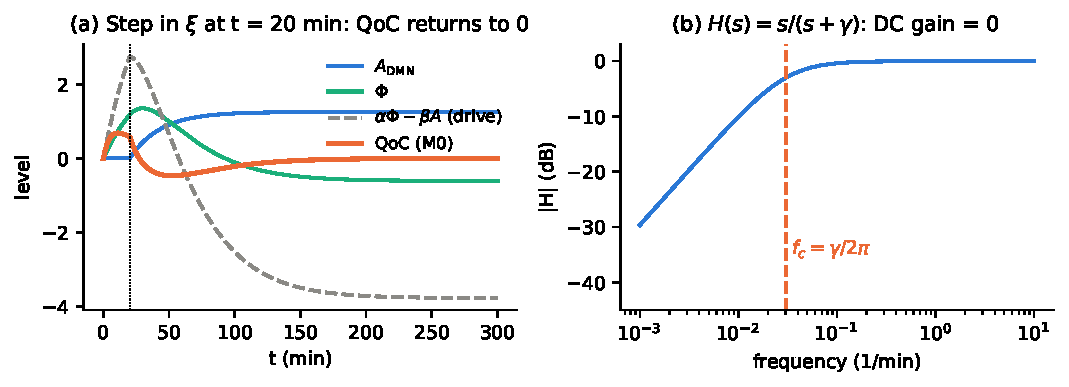
\includegraphics[width=\linewidth]{fig1_highpass_qoc.pdf}
\caption{Mệnh đề~\ref{prop:p2} trên chính ODE \eqref{eq:m0A}--\eqref{eq:m0Q} với tham số in sẵn. (a)~Một bước nhảy của kích thích $\xi$ tại $t=20$~phút đưa $A$ và $\Phi$ sang mức mới và kích thích $\alpha\Phi-\beta A$ về $-3{,}77$; QoC chỉ đáp ứng quá độ rồi trở về không (giá trị cuối $-8\times10^{-9}$, suy giảm $>10^{8}$). (b)~Biên độ Bode của $H(s)=s/(s+\gamma)$: độ lợi không tại DC, tần số góc $\gamma/2\pi$. Kích thích hình sin ở $\omega=0{,}05;\,0{,}2;\,1{,}0$~rad/phút tái tạo $|H(j\omega)|$ với sai số tương đối $0{,}14\,\%$, $0$, $0$.}
\label{fig:highpass}
\end{figure}

\Cref{tab:steady} và \Cref{fig:highpass} tóm tắt Mệnh đề~\ref{prop:p1}--\ref{prop:p3}. Điểm cân bằng của M0 dưới nhiễu kỳ vọng không có $\QoC^*=0$ chính xác, và đáp ứng bước ở \Cref{fig:highpass}a cho thấy đây không phải hiện tượng riêng của một điểm cân bằng: một thay đổi bền vững của hoạt động DMN và tích hợp tạo ra thay đổi bền vững của \emph{kích thích} nhưng không tạo ra QoC bền vững. Các dạng đóng in sẵn khác với điểm cân bằng thật ở cả ba thành phần và phần dư của chúng trong phương trình mô hình cỡ $\gamma\QoC^*_{\mathrm p}\approx5{,}3$ mỗi phút, lớn hơn tốc độ lớn nhất trong mô hình hai bậc độ lớn.

\begin{figure}[t]
\centering
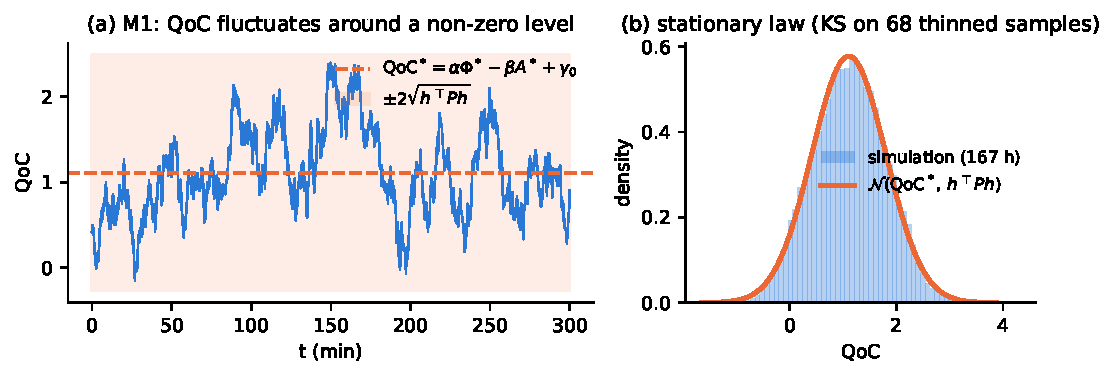
\includegraphics[width=\linewidth]{fig2_m1_stationary.pdf}
\caption{Mệnh đề~\ref{prop:p4}--\ref{prop:p5} cho M1 tại tham số danh nghĩa. (a)~Một đoạn 300 phút của phiên mô phỏng (rời rạc hoá chính xác, $\Delta=10$~s) dao động quanh $\QoC^*=1{,}108$; dải là $\pm2\sqrt{\hv^\top P\hv}$. (b)~Histogram của QoC trên mô phỏng $10^4$ phút so với luật dạng đóng $\mathcal N(\QoC^*,\hv^\top P\hv)$ (tiêu đề panel đếm số mẫu thưa của riêng lần chạy này). Cổng kiểm tra dùng kiểm định Kolmogorov--Smirnov trên 2\,000 mẫu thưa (một mẫu mỗi năm hằng số thời gian chậm nhất) gộp từ năm chuỗi độc lập: $D=0{,}020$, $p=0{,}42$; sai số của trung bình mẫu và độ lệch chuẩn mẫu $0{,}005$ và $0{,}007$.}
\label{fig:stationary}
\end{figure}

M1 khắc phục khiếm khuyết này (\Cref{fig:stationary}). Phần dư Lyapunov của \eqref{eq:P} bằng không tới độ chính xác máy, mức dừng là $\QoC^*=1{,}108$ với phương sai $0{,}477$, và luật dừng thực nghiệm của một mô phỏng dài không phân biệt được với luật Gauss dự đoán. Việc gộp nhiều chuỗi độc lập cho kiểm định Kolmogorov--Smirnov là có chủ ý: một đường đơn của quá trình tự tương quan có thể nằm cách kỳ vọng hai đến ba sai số chuẩn suốt hàng trăm mẫu thưa (một trong mười hai seed được khảo sát cho $z=3{,}5$ khi đứng riêng; độ lệch chuẩn của $z$ trên các seed là $0{,}99$, tức không chệch), và một cổng kiểm tra không được phụ thuộc vào may rủi của một seed.

\subsection{Khả năng xác định tham số}
\label{sec:res-ident}

\paragraph{Cấu trúc.} \Cref{tab:structural} cho hạng của ma trận thông tin chính xác ở bốn cấu hình quan sát. Chỉ với điểm tự chấm, sáu trong mười tham số đi vào hàm hợp lý là xác định được; bốn hướng là null và cách khắc phục thực tế là cố định $A_0$, $\alpha$, $\sA$ và $\kint$, tức từ bỏ thang đo của cả hai biến ẩn và mức nền. Thêm một kênh EEG chỉ còn đúng một hướng null, và trong cả hai trường hợp đó là một đối xứng chính xác của mô hình (\Cref{app:symmetry}): khi không quan sát $\Phi$, phép $(\kint,\sPhi,\alpha)\mapsto(c\,\kint,c\,\sPhi,\alpha/c)$ giữ nguyên luật của mọi quan sát (thang đo của $\Phi$ là tuỳ ý); khi không quan sát $A$, phép affine $A\mapsto cA+(1-c)\Amax$ với $(\kint,A_0,\sA,\beta,\gamma_0)\mapsto(\kint/c,\;cA_0+(1-c)\Amax,\;c\sA,\;\beta/c,\;\gamma_0+\beta(1-c)/c)$ cũng vậy (thang đo của $A$ chỉ được neo bởi $\Amax$). Các vectơ null tính bằng số trùng với gradient của các họ một tham số này. Chỉ cấu hình (d), điểm tự chấm cùng cả hai kênh EEG, xác định đủ 12 tham số, với ma trận thông tin điều kiện tốt (số điều kiện 188 sau chuẩn hoá).

\begin{table}[t]
\centering\small
\caption{Khả năng xác định cấu trúc theo tiêu chí hạng Rothenberg (phiên 90 phút, hỏi mỗi phút, $\gamma_0=0{,}3$). ``Vắng'': tham số không đi vào hàm hợp lý. Hướng null của (b) và (c) là các đối xứng chính xác ở \Cref{app:symmetry}. Cột cuối nêu tham số phải cố định để khôi phục khả năng xác định cục bộ.}
\label{tab:structural}
\footnotesize\setlength{\tabcolsep}{4pt}
\begin{tabular}{llcll}
\toprule
Cấu hình & Vắng & Hạng & Hướng null & Cố định \\
\midrule
(a) điểm tự chấm                 & $\rA,\rPhi$ & 6/10  & bốn (các đối xứng dưới $+$ thang nhiễu) & $A_0,\alpha,\sA,\kint$ \\
(b) điểm tự chấm $+\,y_A$        & $\rPhi$     & 10/11 & co giãn $\Phi$: $\kint,\sPhi\uparrow$, $\alpha\downarrow$ & $\alpha$ \\
(c) điểm tự chấm $+\,y_\Phi$     & $\rA$       & 10/11 & affine $A$: $\gamma_0,\beta,A_0,\kint\uparrow$, $\sA\downarrow$ & $\gamma_0$ \\
(d) điểm tự chấm $+\,y_A+y_\Phi$ & --          & 12/12 & không & không \\
\bottomrule
\end{tabular}
\end{table}

\paragraph{Thực hành.} \Cref{tab:crb} liệt kê CRB tương đối ở thiết kế tham chiếu. Hai điểm đáng lưu ý cho thiết kế. Thứ nhất, ba hằng số tốc độ $\kinh,\kint,\kd$ là các tham số khó nhất ở mọi cấu hình (15--18\,\% ở cấu hình (d), so với 3\,\% cho $A_0$ và 4--7\,\% cho các hệ số khuếch đại). Thứ hai, các kênh EEG làm phần lớn công việc: chỉ điểm tự chấm cho $\CRB(\kinh)=556\,\%$ và $\CRB(\beta)=277\,\%$, tức không có thông tin dùng được, còn một kênh duy nhất đã đưa $\kinh$ về 16--48\,\% tuỳ kênh. Kênh DMN là kênh quan trọng với $\kinh$ và $A_0$ (cấu hình (b) gần tốt bằng (d) cho chúng), kênh $\Phi$ với $\sPhi$ và $\alpha$.

\begin{table}[t]
\centering\small
\caption{Cận Cramér--Rao tương đối theo cấu hình quan sát ở thiết kế tham chiếu ($N=12$, 45 phút, hỏi mỗi 2 phút, $\rA=\rPhi=0{,}1$, $\rQ=0{,}3$). ``cố định'': chuẩn hoá một hướng không xác định được (\Cref{tab:structural}); ``vắng'': tham số không đi vào hàm hợp lý; với $\gamma_0=0$ báo sai số chuẩn tuyệt đối.}
\label{tab:crb}
\begin{tabular}{lcccc}
\toprule
 & (a) điểm tự chấm & (b) $+\,y_A$ & (c) $+\,y_\Phi$ & (d) $+\,y_A+y_\Phi$ \\
\midrule
$\kinh$   & 5,559 & 0,157 & 0,480 & 0,155 \\
$A_0$     & 0,325 & 0,031 & 0,170 & 0,030 \\
$\sA$     & cố định & 0,049 & 0,309 & 0,049 \\
$\kint$   & cố định & 0,260 & 0,254 & 0,175 \\
$\kd$     & 1,155 & 0,337 & 0,372 & 0,178 \\
$\sPhi$   & 8,607 & 0,175 & 0,063 & 0,057 \\
$\alpha$  & cố định & cố định & 0,092 & 0,037 \\
$\beta$   & 2,765 & 0,116 & 0,137 & 0,072 \\
$\gamma_0$& cố định & SE $=0{,}736$ & cố định & SE $=0{,}130$ \\
$\rA$     & vắng & 0,016 & vắng & 0,016 \\
$\rPhi$   & vắng & vắng & 0,014 & 0,014 \\
$\rQ$     & 0,212 & 0,070 & 0,122 & 0,050 \\
\bottomrule
\end{tabular}
\end{table}

\begin{figure}[t]
\centering
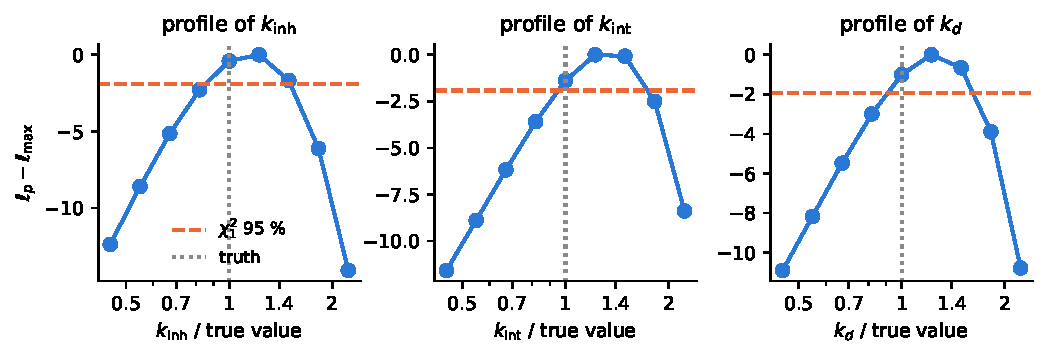
\includegraphics[width=\linewidth]{fig3_profiles.pdf}
\caption{Log-hợp lý profile của ba hằng số tốc độ trên một bộ dữ liệu mô phỏng của thiết kế tham chiếu (cấu hình (d)), mọi tham số khác được tối ưu lại tại mỗi điểm lưới. Đường gạch: ngưỡng 95\,\% của $\chi^2_1$ ($-1{,}92$); đường chấm: giá trị thật. Mỗi profile đơn mốt với cực đại cách giá trị thật không quá một bước lưới ($\kinh$: 0,244 so với 0,200; $\kint$: 0,099 so với 0,081; $\kd$: 0,042 so với 0,034), và độ cong suy ra từ mức sụt 8--14 đơn vị log-hợp lý tại $\pm0{,}8$ đơn vị log tương ứng sai số chuẩn tương đối $0{,}15$--$0{,}20$, phù hợp với cận $0{,}16$--$0{,}18$ ở \Cref{tab:crb}.}
\label{fig:profiles}
\end{figure}

Các profile hợp lý ở \Cref{fig:profiles} xác nhận các hằng số tốc độ xác định được trong thực hành ở cấu hình (d): không profile nào phẳng hay đa mốt trong cửa sổ $\pm0{,}8$ đơn vị log, và các khoảng 95\,\% dựa trên hợp lý có độ rộng nhất quán với cận Fisher.

\subsection{Cận dự đoán được sai số của hợp lý cực đại}
\label{sec:res-crbvalid}

\begin{figure}[t]
\centering
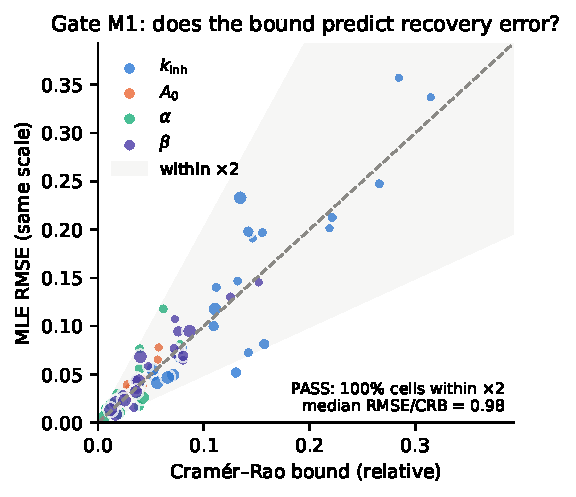
\includegraphics[width=0.55\linewidth]{fig4_crb_vs_mle.pdf}
\caption{Cổng M1. Sai số căn quân phương của phục hồi hợp lý cực đại (năm bộ dữ liệu độc lập mỗi ô, 24 ô thiết kế trải khắp lưới) so với cận Cramér--Rao tương đối, cùng thang; cỡ điểm tăng theo $N$. Vùng tô là hệ số hai quanh đường chéo. Cả 24 ô đạt; tỉ số trung vị $\RMSE/\CRB$ là $0{,}98$ (phân vị 10--90: $0{,}61$--$1{,}40$, cực trị $0{,}40$ và $1{,}93$).}
\label{fig:crbvalid}
\end{figure}

\Cref{fig:crbvalid} so sánh RMSE thực tế của ước lượng ML với CRB ở 24 ô phủ $N$ từ 6 đến 48, phiên từ 20 đến 90 phút, mọi khoảng hỏi và mọi mức nhiễu. Tỉ số $\RMSE/\CRB$ có trung vị $0{,}98$ và trung vị theo tham số $0{,}96$ ($\kinh$), $0{,}97$ ($A_0$), $1{,}00$ ($\alpha$) và $1{,}06$ ($\beta$); không tỉ số nào vượt $2$ và năm tỉ số dưới $0{,}5$ (nhỏ nhất $0{,}40$) là nhiễu lấy mẫu của một RMSE tính từ năm lần fit rơi \emph{dưới} cận, không phải dấu hiệu có vấn đề. Lo ngại rằng cận lạc quan ở $N$ nhỏ không xảy ra: ở bốn ô $N=6$ tỉ số nằm trong khoảng $0{,}7$ đến $1{,}5$. Tại ô tham chiếu, cận dự đoán $(15{,}5;\,3{,}0;\,3{,}7;\,7{,}2)\,\%$ cho $(\kinh,A_0,\alpha,\beta)$ và ML đạt $(19{,}7;\,2{,}6;\,3{,}8;\,7{,}7)\,\%$. Vì vậy chúng tôi dùng CRB chính xác, tốn khoảng hai giây mỗi thiết kế, thay cho mô phỏng để lập toàn bộ bản đồ thiết kế.

\subsection{Bản đồ thiết kế}
\label{sec:res-design}

\begin{figure}[t]
\centering
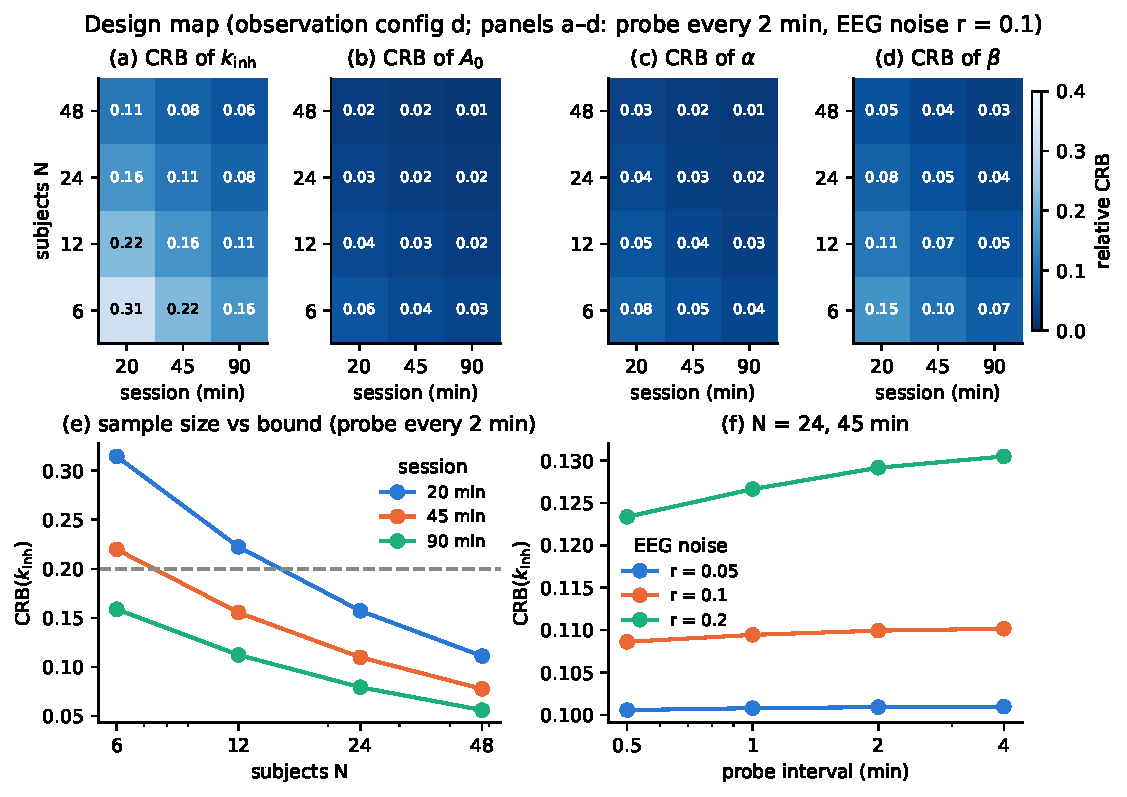
\includegraphics[width=\linewidth]{fig5_design_map.pdf}
\caption{Bản đồ thiết kế (cấu hình (d)). (a--d)~CRB tương đối của $\kinh$, $A_0$, $\alpha$, $\beta$ theo số người và độ dài phiên, với hỏi mỗi 2 phút và nhiễu EEG $r=0{,}1$; ô có giá trị dưới 0,2 là đủ. (e)~$\CRB(\kinh)$ theo $N$ cho ba độ dài phiên; đường gạch là tiêu chí 20\,\%. (f)~Ảnh hưởng của khoảng hỏi và mức nhiễu EEG lên $\CRB(\kinh)$ tại $N=24$, 45 phút: khoảng hỏi không quan trọng với $\kinh$, nhiễu EEG thì có.}
\label{fig:designmap}
\end{figure}

\begin{table}[t]
\centering\small
\caption{Thiết kế rẻ nhất trong lưới ($N\times T$ nhỏ nhất, hoà thì xét cận) có CRB tương đối $\le 20\,\%$ cho từng tham số chính, và tỉ lệ ô trong 144 ô của lưới là đủ cho tham số đó.}
\label{tab:mindesign}
\begin{tabular}{lrrrrrr}
\toprule
Tham số & $N$ & phiên (phút) & hỏi (phút) & nhiễu EEG $r$ & CRB & ô đủ \\
\midrule
$\kinh$  & 24 & 20 & 0,5 & 0,05 & 0,142 & 75\,\% \\
$A_0$    & 6  & 20 & 0,5 & 0,05 & 0,057 & 100\,\% \\
$\alpha$ & 6  & 20 & 0,5 & 0,05 & 0,037 & 100\,\% \\
$\beta$  & 6  & 20 & 0,5 & 0,05 & 0,072 & 98\,\% \\
\bottomrule
\end{tabular}
\end{table}

\Cref{fig:designmap} và \Cref{tab:mindesign} là kết quả thực hành trung tâm. Ba điểm nổi bật.

\emph{Tốc độ ức chế DMN là nút thắt.} $A_0$ và $\alpha$ được ước lượng đủ ở cả 144 thiết kế, $\beta$ ở tất cả trừ ba thiết kế nhỏ nhất (6 người, 20 phút, hỏi mỗi 4 phút), trong khi $\kinh$ đủ ở 75\,\% số thiết kế và không đạt ở mọi thiết kế 6 người ngắn hơn 90 phút (xấu nhất $38\,\%$ tại $N=6$, 20 phút, $r=0{,}2$). Với hỏi mỗi 2 phút và phiên 45 phút, $N=12$ đạt $14{,}3$--$15{,}5\,\%$ cho $\kinh$ khi $r\le0{,}1$ và $18{,}3\,\%$ khi $r=0{,}2$, còn $N=6$ cho $22\,\%$.

\emph{Quy tắc co giãn đơn giản.} Hồi quy log-tuyến tính của cận theo các biến thiết kế trên 144 ô (\Cref{tab:scaling}) cho thấy mọi cận co giãn đúng như $N^{-1/2}$, như bắt buộc với các người tham gia độc lập, và gần như $T^{-1/2}$ theo độ dài phiên; số mũ của $T$ yếu hơn một chút với $\kinh$ ($-0{,}46$) và $A_0$ ($-0{,}39$) vì mỗi người mới đóng góp một mẫu độc lập từ luật dừng trong khi thêm phút của cùng một người lại tự tương quan. Do đó nhiều phiên ngắn tốt hơn một chút so với ít phiên dài đối với các tham số DMN và tương đương đối với các hệ số khuếch đại: cùng $NT$, 24 $\times$ 20 phút cho $\CRB(A_0)=2{,}9\,\%$ so với $3{,}2\,\%$ của 6 $\times$ 90 phút. Các biến thiết kế còn lại tác động khác nhau lên từng tham số: khoảng hỏi không ảnh hưởng $\kinh$ và $A_0$ (được cung cấp thông tin bởi kênh EEG dày) nhưng đi vào các hệ số $\alpha,\beta$ với số mũ $\approx0{,}45$, tức giảm một nửa khoảng hỏi giảm cận của chúng khoảng 27\,\%; nhiễu EEG ảnh hưởng $\kinh$ và các hệ số khuếch đại với số mũ $\approx0{,}17$--$0{,}20$ và không ảnh hưởng $A_0$. Với $\kinh$, quy tắc gần như rút về một yêu cầu tổng thời gian ghi: ở $r\le0{,}1$ khoảng $480$--$540$ phút-người EEG hai kênh (24 $\times$ 20 phút, 12 $\times$ 45 phút hoặc 6 $\times$ 90 phút) đưa cận về 15--16\,\%.

\begin{table}[t]
\centering\small
\caption{Số mũ của hồi quy luỹ thừa $\CRB\propto N^{a}\,T^{b}\,r^{c}\,T_p^{d}$ trên 144 ô của lưới (bình phương tối thiểu log-tuyến tính; $N$ số người, $T$ độ dài phiên, $r$ độ lệch chuẩn nhiễu EEG, $T_p$ khoảng hỏi).}
\label{tab:scaling}
\begin{tabular}{lrrrr}
\toprule
Tham số & $a$ (số người) & $b$ (độ dài phiên) & $c$ (nhiễu EEG) & $d$ (khoảng hỏi) \\
\midrule
$\kinh$  & $-0{,}50$ & $-0{,}46$ & $0{,}17$ & $0{,}01$ \\
$A_0$    & $-0{,}50$ & $-0{,}39$ & $0{,}02$ & $0{,}00$ \\
$\alpha$ & $-0{,}50$ & $-0{,}50$ & $0{,}17$ & $0{,}44$ \\
$\beta$  & $-0{,}50$ & $-0{,}50$ & $0{,}20$ & $0{,}45$ \\
\bottomrule
\end{tabular}
\end{table}

\emph{Lịch hỏi.} Với 22 lần hỏi trong phiên 45 phút, lịch đều đạt tiêu chí Ds nhỏ nhất trong mọi lịch đã thử. Các đối thủ gần nhất, dồn đầu hoặc dồn cuối nhẹ ($p=0{,}85$ và $1{,}15$), chỉ cách nó $0{,}05\,\%$ về trung bình nhân sai số chuẩn; dồn đầu mạnh ($p=0{,}4$) tốn $1{,}2\,\%$, và hỏi theo cặp cách một epoch tốn $4{,}6\,\%$ (cặp cách 12 epoch $0{,}4\,\%$). Dồn cuối mạnh ($p\ge2{,}2$) làm các lần hỏi trùng epoch nên không khả thi. Chúng tôi không tuyên bố tối ưu toàn cục trên mọi lịch; kết quả là lịch đều thông dụng không thua các lịch không đều thường gặp, vì ở cấu hình (d) động lực nhanh đã được các kênh EEG phân giải và điểm tự chấm chủ yếu cung cấp thông tin cho các hệ số khuếch đại tĩnh, với chúng việc trải đều các lần hỏi là tự nhiên.

\subsection{Điều khiển vòng kín}
\label{sec:res-control}

\begin{figure}[t]
\centering
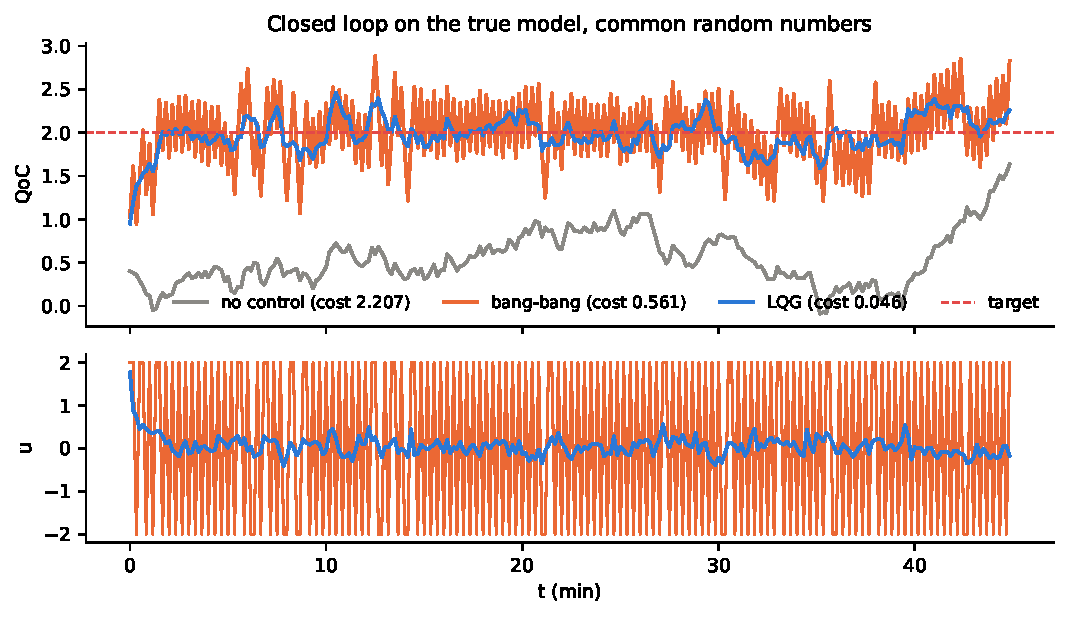
\includegraphics[width=\linewidth]{fig6_control_trajectories.pdf}
\caption{Một phiên vòng kín 45 phút trên mô hình thật với cùng số ngẫu nhiên cho ba chính sách (mục tiêu $\QoC_{\mathrm{tgt}}=2{,}0$, $|u|\le2$). Trên: QoC; dưới: đầu vào $u$. LQG giữ QoC ở mục tiêu với đầu vào nhỏ và trơn; bang-bang dao động giữa $\pm u_{\max}$ và vượt mục tiêu; không điều khiển, QoC dao động quanh $\QoC^*=1{,}1$.}
\label{fig:control}
\end{figure}

\begin{table}[t]
\centering\small
\caption{So sánh chính sách trên mô hình thật (270 epoch, 20 lần thử, cùng số ngẫu nhiên). Chi phí $=\overline{(\QoC-\QoC_{\mathrm{tgt}})^2}+0{,}1\,\overline{u^2}$. Dòng cuối là giá trị dừng dạng đóng của vòng LQG không cắt (\Cref{app:lqg}); mô phỏng dài tương ứng cho $0{,}0346$ (lệch 3\,\%).}
\label{tab:policies}
\begin{tabular}{lrrr}
\toprule
Chính sách & Chi phí & MSE bám mục tiêu & RMS đầu vào \\
\midrule
LQG (tham số thật) & 0,039 & 0,035 & 0,22 \\
Bang-bang (cùng bộ ước lượng) & 0,561 & 0,162 & 2,00 \\
Không điều khiển & 1,481 & 1,481 & 0 \\
\midrule
LQG, dạng đóng dừng & 0,034 & 0,030 & 0,18 \\
\bottomrule
\end{tabular}
\end{table}

\Cref{fig:control} và \Cref{tab:policies} tóm tắt cổng M2. Với tham số thật, LQG đạt chi phí phiên thấp hơn 14 lần so với bang-bang và 38 lần so với không điều khiển. Hai chỉ số trung lập kể cùng một câu chuyện: LQG bám mục tiêu với sai số bình phương trung bình $0{,}035$ (khoảng 7\,\% phương sai vòng hở) trong khi dùng đầu vào RMS $0{,}22$, còn bang-bang bám với sai số $0{,}16$ với cái giá là bão hoà cơ cấu chấp hành liên tục. Đầu vào trung bình cần thiết nhỏ ($u_{\mathrm{ss}}=0{,}024$) vì mục tiêu chỉ cao hơn mức vòng hở $0{,}9$ đơn vị; chi phí của LQG bị chi phối bởi tác động không thể giảm của nhiễu quá trình trong một epoch, đó là lý do chi phí dừng dạng đóng ($0{,}034$) gần với giá trị chân trời hữu hạn. Phép so sánh dùng chi phí bậc hai mà LQG cực tiểu; vấn đề không phải bang-bang là nghiệm tồi của bài toán \emph{của nó}, mà là một bộ điều tiết dựa trên mô hình, khai thác ước lượng trạng thái và động lực đã biết, hiệu quả hơn hẳn trong việc giữ một mức, vốn là mục tiêu tự nhiên của vòng neurofeedback.

\begin{figure}[t]
\centering
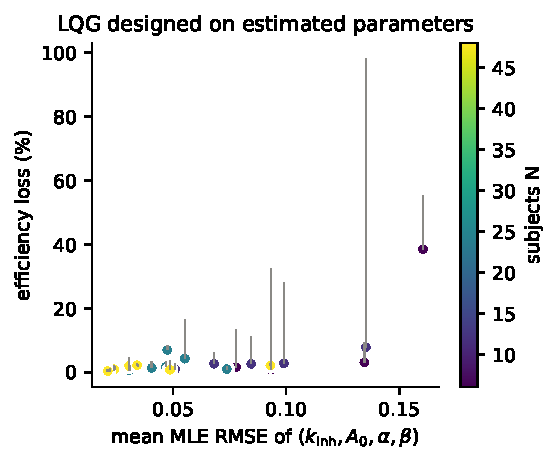
\includegraphics[width=0.6\linewidth]{fig7_robustness.pdf}
\caption{Độ bền của LQG với sai số ước lượng tham số. Với mỗi ô trong 24 ô thiết kế, một bộ điều khiển (độ lợi và bộ lọc) được thiết kế trên từng bộ trong năm bộ tham số ML phục hồi được ở ô đó và chạy trên mô hình thật của ô. Điểm: mất mát hiệu quả trung vị trên các lần fit; râu kéo tới phân vị 90; màu: số người; trục hoành: RMSE tương đối trung bình của $(\kinh,A_0,\alpha,\beta)$ ở ô đó. Giá trị đầy đủ ở \Cref{tab:robust}.}
\label{fig:robustness}
\end{figure}

\Cref{fig:robustness} nối bản đồ thiết kế với điều khiển. Khi bộ điều khiển được thiết kế trên tham số ước lượng từ một thiết kế đủ cho $\kinh$ (19 trong 24 ô), mất mát hiệu quả trung vị chỉ vài phần trăm: $2{,}6\,\%$ (phân vị 90: $11\,\%$) ở thiết kế tham chiếu, $1{,}8\,\%$ ($3{,}4\,\%$) với 24 người $\times$ 45 phút, dưới $1\,\%$ (phân vị 90 $\le 2{,}1\,\%$) với mọi thiết kế 48 người ở $r=0{,}05$, và nhiều nhất $7\,\%$ (phân vị 90 nhiều nhất $17\,\%$) trên toàn bộ các ô đủ. Các mất mát lớn đều đến từ năm ô không đủ: 6 người $\times$ 20 phút với hỏi mỗi 2 phút mất $38\,\%$ ở trung vị và $55\,\%$ ở phân vị 90, còn 12 người $\times$ 20 phút ở $r=0{,}2$ có mất mát trung vị $8\,\%$ nhưng phân vị 90 lên tới $98\,\%$---cứ mười bộ điều khiển thiết kế từ dữ liệu như vậy thì một bộ làm chi phí tăng gấp đôi (hai ô không đủ khác có trung vị vừa phải nhưng phân vị 90 là $28$--$32\,\%$). Vì vậy một thiết kế không ước lượng được mô hình cũng không thể làm nền cho vòng neurofeedback dựa trên mô hình, và tiêu chí 20\,\% ở \Cref{sec:res-design}, với xấp xỉ tốt, chính là ranh giới giữa các bộ điều khiển chỉ mất vài phần trăm và các bộ có thể mất phần lớn lợi ích.

\subsection{Độ nhạy toàn cục}
\label{sec:res-sens}

\begin{figure}[t]
\centering
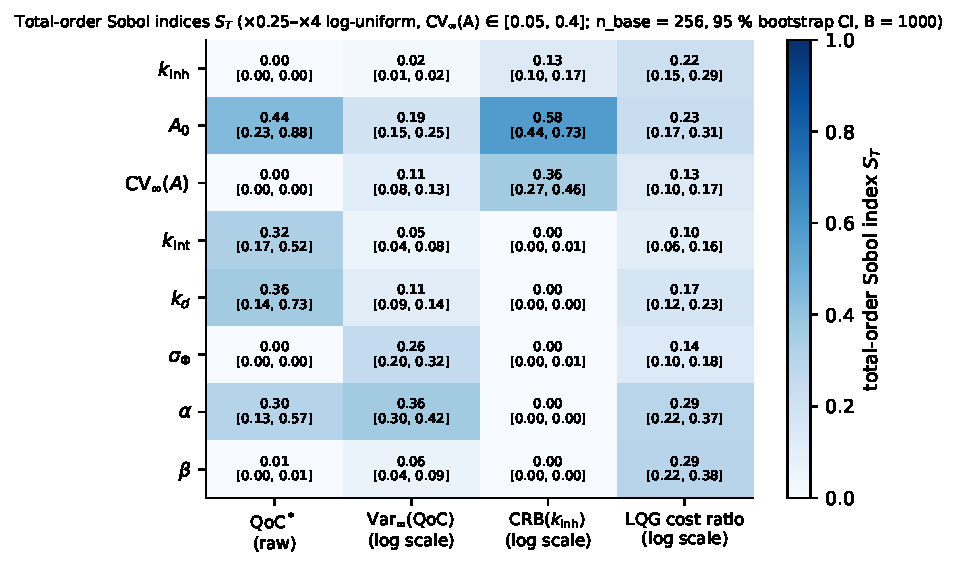
\includegraphics[width=0.8\linewidth]{fig8_sobol.pdf}
\caption{Chỉ số Sobol toàn phần $S_T$ (với khoảng bootstrap 95\,\%) của bốn đầu ra theo tám tham số mô hình quét log-đều trên $\times0{,}25$--$\times4$ quanh điểm danh nghĩa ($\mathrm{CV}_A\in[0{,}05,0{,}4]$). $\Var_\infty(\QoC)$, $\CRB(\kinh)$ và hiệu quả LQG phân tích trên thang log; $\QoC^*$ trên thang thô. Lấy mẫu Sobol có xáo trộn, $n=256$, $2\,560$ lần đánh giá.}
\label{fig:sobol}
\end{figure}

\begin{table}[t]
\centering\small
\caption{Chỉ số Sobol toàn phần $S_T$ với khoảng tin cậy bootstrap 95\,\% ($B=1\,000$). Dòng cuối là chẩn đoán hội tụ $\max_i|\Delta S_{T,i}|$ giữa toàn bộ mẫu và nửa đầu của nó.}
\label{tab:sobol}
\footnotesize\setlength{\tabcolsep}{4pt}
\begin{tabular}{lcccc}
\toprule
Đầu vào & $\QoC^*$ (thô) & $\log\Var_\infty(\QoC)$ & $\log\CRB(\kinh)$ & $\log$ hiệu quả LQG \\
\midrule
$\kinh$          & 0,00 & 0,02 [0,01; 0,02] & 0,13 [0,10; 0,17] & 0,22 [0,15; 0,29] \\
$A_0$            & 0,44 [0,23; 0,88] & 0,19 [0,15; 0,25] & \textbf{0,58} [0,44; 0,73] & 0,23 [0,17; 0,31] \\
$\mathrm{CV}_A$  & 0,00 & 0,11 [0,08; 0,13] & \textbf{0,36} [0,27; 0,46] & 0,13 [0,10; 0,17] \\
$\kint$          & 0,32 [0,17; 0,52] & 0,05 [0,04; 0,08] & 0,00 & 0,10 [0,06; 0,16] \\
$\kd$            & 0,36 [0,14; 0,73] & 0,11 [0,09; 0,14] & 0,00 & 0,17 [0,12; 0,23] \\
$\sPhi$          & 0,00 & 0,26 [0,20; 0,32] & 0,00 & 0,14 [0,10; 0,18] \\
$\alpha$         & 0,30 [0,13; 0,57] & \textbf{0,36} [0,30; 0,42] & 0,00 & 0,29 [0,22; 0,37] \\
$\beta$          & 0,01 [0,00; 0,01] & 0,06 [0,04; 0,09] & 0,00 & 0,29 [0,22; 0,38] \\
\midrule
$\max|\Delta S_T|$ (nửa mẫu) & 0,10 & 0,013 & 0,076 & 0,030 \\
\bottomrule
\end{tabular}
\end{table}

\Cref{fig:sobol} và \Cref{tab:sobol} cho biết các kết luận phụ thuộc vào tham số nào.

\emph{Khả năng xác định $\kinh$ do mức nền DMN và độ biến thiên của nó quyết định, không do $\kinh$.} Chỉ số toàn phần của $A_0$ lên $\log\CRB(\kinh)$ là $0{,}58$ và của $\mathrm{CV}_A$ là $0{,}36$, trong khi chính $\kinh$ chỉ đóng góp $0{,}13$ và năm tham số còn lại không đóng góp gì. Chỉ số bậc nhất ($0{,}46$ và $0{,}25$) nhỏ hơn chỉ số toàn phần, phản ánh tương tác $A_0\times\mathrm{CV}_A$: cái mà kênh EEG phân giải là biên độ dao động DMN, $\mathrm{CV}_A\cdot A_0$, so với nhiễu quan sát. Với người làm thực nghiệm, điều này nghĩa là yêu cầu cỡ mẫu cho $\kinh$ phụ thuộc vào tỉ số tín hiệu trên nhiễu của đặc trưng DMN nhiều hơn hẳn giá trị (chưa biết) của chính tốc độ, và cải thiện đặc trưng DMN đáng giá hơn thêm lần hỏi.

\emph{Độ biến thiên dừng do hệ số khuếch đại $\alpha$ và nhiễu $\Phi$ chi phối.} $\log\Var_\infty(\QoC)$ có $S_T=0{,}36$ với $\alpha$, $0{,}26$ với $\sPhi$ và $0{,}19$ với $A_0$; các chỉ số gần cộng tính ($S_1\approx S_T$) và đã hội tụ ($\max|\Delta S_T|=0{,}013$).

\emph{Hiệu quả điều khiển không có tham số chi phối.} Tỉ số chi phí LQG trải độ nhạy lên $\beta,\alpha,A_0,\kinh,\kd$ ($S_T$ từ $0{,}17$ đến $0{,}29$) với chỉ số bậc nhất nhỏ, tức lợi ích của điều khiển vòng kín là tính chất chung của các hệ số khuếch đại và động lực DMN; không tham số đơn lẻ nào quyết định được nó trong dải khảo sát.

\emph{Mức dừng $\QoC^*$} phụ thuộc $A_0,\kd,\kint,\alpha$ và không phụ thuộc $\beta$ (vì $\QoC^*=\alpha\kint(1-A_0)/\kd-\beta A_0$ và số hạng đầu chiếm ưu thế). Tổng các chỉ số của nó lớn hơn một và khoảng tin cậy rộng (hội tụ $0{,}10$) vì đầu ra là tích của các đầu vào trên thang thô; chúng tôi chỉ giữ lại thứ tự.

%% ─────────────────────────────────────────────────────────────────────────────
\section{Thảo luận}
\label{sec:discussion}

\paragraph{Một phép kiểm tra nhất quán nên đi trước việc fit.} Kết quả đầu tiên là phủ định nhưng, theo chúng tôi, có ích vượt ra ngoài mô hình cụ thể: một phương trình vi phân trong đó biến ``ý thức'' chỉ được dẫn động bởi đạo hàm theo thời gian của các đầu vào thì không thể biểu diễn một trạng thái duy trì, dù tham số thế nào. Thay một trạng thái dừng đề xuất ngược vào phương trình mô hình (Mệnh đề~\ref{prop:p3}) là một phép tính ngắn mà chúng tôi khuyến nghị làm bước thường quy trước khi fit bất kỳ mô hình nào như vậy. Mô hình đã sửa M1 giữ câu chuyện cơ chế của M0---tập luyện ức chế DMN, sự rút lui của DMN nuôi tích hợp, cả hai nuôi chất lượng được báo cáo---nhưng biến nó thành một quá trình ngẫu nhiên dừng đặt đúng với mô-men dạng đóng. Việc nó tuyến tính--Gauss là một lựa chọn mô hình hoá có lợi ích lớn: nó làm cho hàm hợp lý, thông tin Fisher và bộ điều khiển tối ưu đều chính xác, điều cho phép một phân tích thiết kế đầy đủ mà không cần mô phỏng.

\paragraph{Thiết kế lấy mẫu trải nghiệm làm được và không làm được gì.} Phân tích khả năng xác định cho một thứ bậc rõ ràng. Chỉ điểm tự chấm không đủ để học động lực: không có kênh EEG thì thang đo của cả hai biến ẩn là tuỳ ý và các hằng số tốc độ chỉ biết tới hệ số vài lần. Một kênh EEG loại bỏ mọi đối xứng trừ một, và đối xứng đó diễn giải được (biến không quan sát có thể co giãn). Hai kênh xác định mọi thứ. Trong cấu hình xác định được, bản đồ thiết kế và quy tắc co giãn ở \Cref{tab:scaling} chuyển thành lời khuyên dùng được ngay: (i) số lần hỏi chi phối độ chính xác của các hệ số khuếch đại nối trạng thái ẩn với báo cáo, với lợi ích kiểu căn bậc hai; (ii) độ chính xác của hằng số tốc độ DMN phụ thuộc tổng lượng EEG ghi được và chất lượng đặc trưng DMN, không phụ thuộc tần suất hỏi; (iii) khoảng tám giờ-người EEG hai kênh với nhiễu đặc trưng 10\,\% thang tín hiệu đưa hằng số tốc độ về sai số tương đối 15\,\%, còn nghiên cứu sáu người với phiên dưới 90 phút thì không; (iv) lịch hỏi đều là mặc định an toàn. Các phát biểu này nói về một mô hình, không phải về não, nhưng chính là loại phát biểu phải có trước khi chạy một nghiên cứu nếu nghiên cứu đó nhằm ước lượng một mô hình động lực, và chúng vắng bóng trong tài liệu hiện nay về mô hình tính toán của thiền \citep{Laukkonen2021,SandvedSmith2021}, vốn cho đến nay mang tính mô tả.

\paragraph{Từ ước lượng đến can thiệp.} Phân tích điều khiển cho thấy một mô hình mang lại gì một khi đã xác định được. Một bộ điều tiết dùng ước lượng trạng thái và động lực đã biết giữ đại lượng được báo cáo ở mục tiêu với đầu vào nhỏ hơn một bậc so với chính sách ngưỡng và sai số bám nhỏ hơn hơn bốn lần, và hiệu năng của nó dự đoán được ở dạng đóng. Quan trọng hơn, \Cref{fig:robustness} định lượng cái giá của sai số ước lượng bằng chính đơn vị của ứng dụng: bộ điều khiển thiết kế từ thiết kế đủ chỉ mất vài phần trăm, bộ thiết kế từ thiết kế không đủ có thể mất phần lớn lợi ích. Điều này cho tiêu chí xác định được 20\,\% một ý nghĩa vận hành và ủng hộ việc coi thiết kế nghiên cứu ước lượng và thiết kế giao thức neurofeedback là một bài toán, phù hợp với các lời kêu gọi gần đây về phương pháp luận neurofeedback chặt chẽ hơn \citep{Ros2020,Sitaram2017}.

\paragraph{Độ bền của các kết luận.} Phân tích độ nhạy cho thấy khó khăn trong ước lượng $\kinh$ không phải đặc thù của điểm danh nghĩa: trên dải 16 lần của mọi tham số, nó bị chi phối bởi mức nền và hệ số biến thiên của DMN, cả hai đều là tính chất của đặc trưng EEG chứ không phải của tốc độ. Các kết luận về hiệu quả điều khiển và độ biến thiên dừng cũng trải trên nhiều tham số thay vì phụ thuộc một tham số.

\subsection{Hạn chế}
\label{sec:limitations}

\begin{itemize}
  \item \textbf{Không fit dữ liệu thật.} Bài trả lời câu hỏi đi trước phân tích dữ liệu---thiết kế nào đủ để fit mô hình---và không tuyên bố gì về giá trị tham số ở người tập. Điểm danh nghĩa là điểm làm việc; phân tích độ nhạy phủ một dải rộng quanh nó nhưng không phủ các chế độ khác về chất.
  \item \textbf{Tuyến tính và Gauss.} M1 tuyến tính với nhiễu Gauss cộng tính và hàm đọc ra tuyến tính, và điểm tự chấm được coi là liên tục. Điểm tự chấm thật là thứ bậc và bị chặn, mức DMN nằm trong $[0,\Amax]$, và động lực thiền có thể gồm các chuyển trạng thái rời rạc \citep{Hasenkamp2012,Christoff2016}. Mở rộng phi tuyến (hàm đọc ra bão hoà, nhiễu phụ thuộc trạng thái, chuyển chế độ) sẽ cần bộ lọc xấp xỉ và thông tin Fisher dựa trên mô phỏng; phân tích hiện tại là đường cơ sở chính xác để so sánh các mở rộng như vậy.
  \item \textbf{Ánh xạ từ đặc trưng EEG sang $(A,\Phi)$} được giả định, với mức nhiễu là biến thiết kế. Thiết lập ánh xạ đó là việc thực nghiệm; kết quả của chúng tôi cho biết nó phải tốt đến đâu ($r\lesssim0{,}1$--$0{,}2$ thang tín hiệu) để động lực xác định được.
  \item \textbf{Bản đồ thiết kế được biểu diễn theo phút ở tốc độ danh nghĩa.} Độ dài phiên 20--90 phút tương ứng 4--18 hằng số thời gian DMN ở $\kinh=0{,}2$ nhưng chỉ 0,9--3,9 ở giá trị in sẵn $0{,}043\ \mathrm{phút^{-1}}$. Phân tích độ nhạy cho thấy $\CRB(\kinh)$ chỉ phụ thuộc yếu vào chính $\kinh$ trong $\times0{,}25$--$\times4$ ($S_T=0{,}13$), nhưng người đọc kỳ vọng động lực DMN chậm hơn nhiều nên quy đổi độ dài phiên theo đơn vị $1/\kinh$ và dự liệu yêu cầu dịch về phía phiên dài hơn.
  \item \textbf{Gánh nặng của việc hỏi chưa được tính.} Hỏi dày (mỗi 30~s) cải thiện các hệ số khuếch đại trong bản đồ nhưng làm gián đoạn chính việc tập mà nó đo; bản đồ cần đọc cùng với một trần số lần hỏi mà giao thức chấp nhận được, điều nằm ngoài mô hình.
  \item \textbf{Tối ưu lịch hỏi} chỉ giới hạn ở hai họ dễ diễn giải; tối ưu tự do trên vị trí các lần hỏi có thể tìm được lịch tốt hơn, dù các chênh lệch nhỏ quan sát được gợi ý ít dư địa cải thiện ở cấu hình (d).
  \item \textbf{Điều khiển} giả định đầu vào cộng tính vào phương trình DMN với độ lợi đã biết, chấp hành hoàn hảo trong giới hạn và không trễ, và so sánh chính sách trên chi phí bậc hai. Phân tích độ bền phủ sai số tham số nhưng không phủ sai cấu trúc mô hình.
  \item \textbf{Khác biệt giữa người} không được mô hình hoá: mọi người dùng chung một vectơ tham số. Mở rộng phân cấp sẽ thay đổi bản đồ thiết kế về lượng (nhiều người hơn, phiên ngắn hơn) nhưng không thay đổi cấu trúc khả năng xác định.
\end{itemize}

\section{Kết luận}
\label{sec:conclusion}

Với một mô hình DMN--$\Phi$--QoC của động lực thiền mới được đề xuất, chúng tôi đã chỉ ra dạng gốc không có QoC duy trì, đề xuất mô hình tuyến tính--Gauss thay thế với hành vi dừng dạng đóng, xác lập chính xác cấu hình quan sát nào xác định được tham số, kiểm chứng cận Cramér--Rao bằng hợp lý cực đại trên toàn không gian thiết kế, rút ra bản đồ thiết kế định lượng và quy tắc co giãn cho số người, độ dài phiên, khoảng hỏi và chất lượng EEG, đặt và giải bài toán điều khiển vòng kín, và định lượng sai số ước lượng từ mỗi thiết kế lan truyền ra hiệu năng điều khiển như thế nào. Sự kết hợp giữa thông tin Fisher chính xác, các cổng kiểm tra bằng máy và một lệnh tái tạo duy nhất, theo chúng tôi, là một khuôn mẫu cho cách các mô hình động lực của trạng thái tâm trí nên được khảo sát trước khi đem đến dữ liệu.

%% ─────────────────────────────────────────────────────────────────────────────
\section*{Dữ liệu và mã nguồn}
Không dùng dữ liệu thực nghiệm. Mọi kết quả được sinh \emph{in silico} bằng mã Python đi kèm (các mô-đun \path{bqi/dmn_ode.py}, \path{model/}, \path{eeg/model_fit.py} và \path{experiments/run_model_paper.py}) với seed 42; bản chụp cấu hình đầy đủ, kết quả thô, hồ sơ các cổng và hình nằm trong kho mã dưới \path{outputs/}. Kho mã và bản lưu trữ đóng băng có DOI sẽ được công khai khi bài được chấp nhận.

\section*{Lời cảm ơn}
Nghiên cứu được thực hiện tại Trường Đại học Phenikaa, Hà Nội. Mọi tính toán chạy trên máy tính cá nhân; không nhận tài trợ bên ngoài. % TODO: bổ sung tài trợ hoặc mã số đề tài nếu có.

\section*{Đóng góp của tác giả}
D.V.\ hình thành ý tưởng nghiên cứu, xây dựng phương pháp và phần mềm, thực hiện phân tích và viết bản thảo.

\section*{Tuyên bố về xung đột lợi ích}
Tác giả tuyên bố không có xung đột lợi ích. Tác giả cũng là tác giả của mô hình gốc được khảo sát trong bài \citep{BQI}; các sửa đổi ở \Cref{sec:m0wrong} được báo cáo ở đây như một phần của phân tích hiện tại.

%% ─────────────────────────────────────────────────────────────────────────────
\appendix
\section{Chứng minh Mệnh đề~\ref{prop:p1}--\ref{prop:p5}}
\label{app:proofs}

\begin{proof}[Chứng minh Mệnh đề~\ref{prop:p1}]
Tại điểm cân bằng với kích thích hằng $\bar\xi$, \eqref{eq:m0A} cho $A^*=\kspont\bar\xi/\kinh$ và \eqref{eq:m0Phi} cho $\Phi^*=(\kint/\kd)(1-A^*/\Amax)$. Với $\dot A=\dot\Phi=0$, \eqref{eq:m0Q} rút về $0=-\gamma\QoC^*$, nên $\QoC^*=0$ vì $\gamma>0$. Hệ tuyến tính là tam giác dưới với đường chéo âm $(-\kinh,-\kd,-\gamma)$, nên điểm cân bằng là duy nhất và ổn định tiệm cận.
\end{proof}

\begin{proof}[Chứng minh Mệnh đề~\ref{prop:p2}]
Đặt $z=\QoC-v$. Từ \eqref{eq:m0Q}, $\dot z=\dot{\QoC}-\dot v=-\gamma\QoC=-\gamma(z+v)$, một phương trình tuyến tính có nghiệm $z(t)=e^{-\gamma t}z(0)-\gamma\int_0^te^{-\gamma(t-s)}v(s)\dd s$; cộng $v(t)$ được \eqref{eq:qocsol}. Lấy biến đổi Laplace của $\dot{\QoC}=\dot v-\gamma\QoC$ với điều kiện đầu bằng không, $s\,\widehat{\QoC}=s\hat v-\gamma\widehat{\QoC}$, nên $H(s)=s/(s+\gamma)$, $H(0)=0$ và $|H(j\omega)|^2=\omega^2/(\omega^2+\gamma^2)$. Nếu $v(t)\to v_\infty$, số hạng tích chập trong \eqref{eq:qocsol} tiến tới $v_\infty$ (vì $\gamma\int_0^te^{-\gamma(t-s)}\dd s\to1$), nên $\QoC(t)\to v_\infty-v_\infty=0$.
\end{proof}

\begin{proof}[Chứng minh Mệnh đề~\ref{prop:p3}]
Thay bất kỳ bộ ba nào có $\dot A=\dot\Phi=0$ vào \eqref{eq:m0Q} được $\dot{\QoC}=-\gamma\QoC$, chỉ triệt tiêu tại $\QoC=0$; theo \eqref{eq:paperss}, $\QoC^*_{\mathrm p}>0$ khi $\alpha,\beta,\kint>0$ và $A^*_{\mathrm p}<\Amax$. Phần dư bằng số suy ra khi thay tham số in sẵn với $\bar\xi=0$: $\dot A=-\kinh A^*_{\mathrm p}=-0{,}043\times0{,}0787=-3{,}4\times10^{-3}$, $\dot\Phi=0$ theo cách dựng $\Phi^*_{\mathrm p}$, và $\dot{\QoC}=-\beta\dot A-\gamma\QoC^*_{\mathrm p}=0{,}0063-0{,}19\times27{,}81=-5{,}277$.
\end{proof}

\begin{proof}[Chứng minh Mệnh đề~\ref{prop:p4}]
Với SDE tuyến tính $\dd\xv=(M\xv+\uv)\dd t+G\dd\mathbf W$ có $M$ Hurwitz, kỳ vọng tuân theo $\dot{\muv}=M\muv+\uv$ và hiệp phương sai $\dot P=MP+PM^\top+GG^\top$ \citep{Gardiner2009}; giá trị dừng giải $M\muv+\uv=0$ và $MP+PM^\top+GG^\top=0$. Giải phương trình đầu với \eqref{eq:ss} được \eqref{eq:m1ss}. Viết phương trình Lyapunov theo từng phần tử với $M$ tam giác dưới: phần tử $(1,1)$ cho $-2\kinh P_{AA}+\sA^2=0$; phần tử $(1,2)$ cho $-\kinh P_{A\Phi}-(\kint/\Amax)P_{AA}-\kd P_{A\Phi}=0$; phần tử $(2,2)$ cho $-2(\kint/\Amax)P_{A\Phi}-2\kd P_{\Phi\Phi}+\sPhi^2=0$. Giải theo thứ tự này được \eqref{eq:P}. Tại tham số danh nghĩa $P_{AA}=0{,}025$, $P_{A\Phi}=-0{,}00865$, $P_{\Phi\Phi}=0{,}0574$ và $\hv^\top P\hv=\beta^2P_{AA}-2\alpha\beta P_{A\Phi}+\alpha^2P_{\Phi\Phi}=0{,}477$. $\QoC^*=0$ xác định một tập đối chiều một trong không gian tham số, nên $\QoC^*\neq0$ với tham số tổng quát.
\end{proof}

\begin{proof}[Chứng minh Mệnh đề~\ref{prop:p5}]
Nghiệm của SDE tuyến tính dẫn động bởi chuyển động Brown từ điều kiện đầu Gauss là một quá trình Gauss; với luật đầu là luật dừng thì quá trình dừng. Với $\tau\ge0$, $\xv(t+\tau)=e^{M\tau}\xv(t)+\int_t^{t+\tau}e^{M(t+\tau-s)}(\uv\dd s+G\dd\mathbf W_s)$, và tích phân độc lập với $\xv(t)$, nên $\Cov(\xv(t+\tau),\xv(t))=e^{M\tau}P$. Một phiếm hàm tuyến tính $\hv^\top\xv+\gamma_0$ của quá trình Gauss là Gauss với kỳ vọng, phương sai và tự hiệp phương sai như đã nêu.
\end{proof}

\section{Các đối xứng chính xác đằng sau hướng null}
\label{app:symmetry}

Gọi $\mathcal L_{\thetav}$ là luật đồng thời của mọi quan sát trong một phiên.

\begin{proposition}[Co giãn $\Phi$, cấu hình (b)]
Nếu không quan sát $y_\Phi$, thì với mọi $c>0$ phép biến đổi tham số $\kint\mapsto c\kint$, $\sPhi\mapsto c\sPhi$, $\alpha\mapsto\alpha/c$ (các tham số khác giữ nguyên) không làm thay đổi $\mathcal L_{\thetav}$.
\end{proposition}
\begin{proof}
Đặt $\Phi'=c\Phi$. Khi đó $\dd\Phi'=[c\kint(1-A/\Amax)-\kd\Phi']\dd t+c\sPhi\dd W_\Phi$, chính là \eqref{eq:m1Phi} với $(c\kint,c\sPhi)$; phương trình $A$ không đổi; và $\QoC=\alpha\Phi-\beta A+\gamma_0=(\alpha/c)\Phi'-\beta A+\gamma_0$. Vì vậy các quá trình quan sát được $A$ (qua $y_A$) và $\QoC$ (qua điểm tự chấm) có cùng luật dưới cả hai vectơ tham số.
\end{proof}

\begin{proposition}[Phép affine $A$, cấu hình (c)]
Nếu không quan sát $y_A$, thì với mọi $c>0$ phép biến đổi
\begin{gather*}
\kint\mapsto\kint/c,\qquad A_0\mapsto cA_0+(1-c)\Amax,\qquad \sA\mapsto c\sA,\\
\beta\mapsto\beta/c,\qquad \gamma_0\mapsto\gamma_0+\beta(1-c)/c
\end{gather*}
không làm thay đổi $\mathcal L_{\thetav}$.
\end{proposition}
\begin{proof}
Đặt $A'=cA+(1-c)\Amax$. Khi đó $\dd A'=c\dd A=-\kinh\bigl(A'-[cA_0+(1-c)\Amax]\bigr)\dd t+c\sA\dd W_A$. Trong phương trình $\Phi$, $\kint(1-A/\Amax)=\kint\bigl(1-(A'-(1-c)\Amax)/(c\Amax)\bigr)=(\kint/c)(1-A'/\Amax)$. Trong hàm đọc ra, $-\beta A=-(\beta/c)A'+\beta(1-c)\Amax/c$, được hấp thụ vào $\gamma_0$ (với $\Amax=1$). Các quá trình quan sát được $\Phi$ và $\QoC$ có cùng luật dưới cả hai vectơ tham số.
\end{proof}

Lấy đạo hàm mỗi họ tại $c=1$ trong toạ độ đã biến đổi (log với tham số dương) được các hướng tiếp tuyến
\begin{gather*}
(\dd\log\kint,\dd\log\sPhi,\dd\alpha)=(1,1,-\alpha),\\
(\dd\log\kint,\dd A_0,\dd\log\sA,\dd\beta,\dd\gamma_0)=(-1,\,A_0-\Amax,\,1,\,-\beta,\,-\beta).
\end{gather*}
Với mỗi tiếp tuyến $\mathbf v$, dạng toàn phương $\mathbf v^\top\mathcal I\mathbf v$ triệt tiêu tới độ chính xác máy ($10^{-16}$ so với $\mathbf v^\top\diag(\mathcal I)\mathbf v$), và sau chuẩn hoá đường chéo ở \Cref{sec:structural}, tiếp tuyến trùng với vectơ null tìm được bằng số (cosin $1{,}000$); các vectơ null chuẩn hoá, sai khác dấu, là
\begin{gather*}
\text{(b)}:\ (\alpha,\kint,\sPhi)=(0{,}709;\,-0{,}619;\,-0{,}337),\\
\text{(c)}:\ (\gamma_0,\beta,A_0,\kint,\sA)=(0{,}767;\,0{,}491;\,0{,}281;\,0{,}250;\,-0{,}170).
\end{gather*} Ở cấu hình (a) cả hai họ đều có mặt, cùng với hai hướng nữa đánh đổi thang nhiễu $\sA,\sPhi$ với các hệ số khuếch đại; cố định $(A_0,\alpha,\sA,\kint)$ loại bỏ cả bốn. Ở cấu hình (d) cả $A$ và $\Phi$ được quan sát trực tiếp, không co giãn nào khả dĩ, và ma trận thông tin có hạng đầy đủ.

\section{Rời rạc hoá Van Loan}
\label{app:vanloan}

Với $n=2$, lập ma trận $2n\times2n$ $V=\begin{pmatrix}-M & GG^\top\\ 0 & M^\top\end{pmatrix}$ và tính $E=e^{V\Delta}=\begin{pmatrix}E_{11}&E_{12}\\0&E_{22}\end{pmatrix}$. Khi đó $F=E_{22}^\top=e^{M\Delta}$ và $Q=E_{22}^\top E_{12}=\int_0^\Delta e^{Ms}GG^\top e^{M^\top s}\dd s$ \citep{VanLoan1978}. Đầu vào tất định được tích phân chính xác thành $\mathbf c=M^{-1}(F-I)\uv$, và ma trận đầu vào điều khiển thành $B=M^{-1}(F-I)\mathbf b$ (giữ bậc không). Hiệp phương sai dừng rời rạc thoả $P=FPF^\top+Q$ và trùng với $P$ liên tục của \eqref{eq:P}, điều được dùng làm unit test.

\section{Bộ lọc Kalman tuần tự}
\label{app:kalman}

Với tiên nghiệm $\hat\xv_{0|0}=\muv$, $P_{0|0}=P$, mỗi epoch gồm bước dự đoán $\hat\xv_{t|t-1}=F\hat\xv_{t-1|t-1}+\mathbf c$, $P_{t|t-1}=FP_{t-1|t-1}F^\top+Q$, rồi một bước cập nhật vô hướng cho mỗi quan sát có sẵn $y=\mathbf s^\top\xv+o+e$, $e\sim\mathcal N(0,r^2)$, với $(\mathbf s,o,r)=(\mathbf e_1,0,\rA)$ cho $y_A$, $(\mathbf e_2,0,\rPhi)$ cho $y_\Phi$ và $(\hv,\gamma_0,\rQ)$ cho điểm tự chấm:
\begin{gather*}
\nu=y-\mathbf s^\top\hat\xv-o,\qquad S=\mathbf s^\top P\mathbf s+r^2,\qquad \mathbf k=P\mathbf s/S,\\
\hat\xv\leftarrow\hat\xv+\mathbf k\nu,\qquad P\leftarrow P-\mathbf k\mathbf k^\top S,\qquad
\ell\mathrel{+}=-\tfrac12\bigl(\log2\pi S+\nu^2/S\bigr).
\end{gather*}
Vì các nhiễu quan sát độc lập, cập nhật vô hướng tuần tự tương đương chính xác với cập nhật vectơ \citep{Durbin2012}; tổng $\ell$ là log-hợp lý chính xác của phiên và bằng log-mật độ Gauss của vectơ xếp chồng ở \Cref{app:fisher}.

\section{Thông tin Fisher chính xác của một phiên}
\label{app:fisher}

Gọi $T$ là số epoch và xếp chồng đường ẩn $\mathbf X=(\xv_1^\top,\dots,\xv_T^\top)^\top\in\R^{2T}$. Dưới tính dừng, $\E\mathbf X=\One_T\otimes\muv$ và $\Cov(\xv_t,\xv_s)=F^{\,t-s}P$ với $t\ge s$ (và chuyển vị với $t<s$), nên $\Sigma_X$ là ma trận khối Toeplitz với các khối $C_k=F^kP$. Mỗi quan sát là $y=\mathbf s^\top\mathbf X+o+e$ với một hàng chọn $\mathbf s$ (vectơ đơn vị cho $y_A,y_\Phi$, hàm đọc ra $\hv$ đặt tại epoch hỏi cho điểm tự chấm); gom các hàng vào $S$, các độ lệch vào $\mathbf o$ và các phương sai nhiễu vào $D$,
\[
\mathbf Y=S\mathbf X+\mathbf o+\mathbf e\sim\mathcal N\bigl(\mathbf m,\Sigma\bigr),\qquad
\mathbf m=S(\One\otimes\muv)+\mathbf o,\qquad \Sigma=S\Sigma_XS^\top+D .
\]
Phương trình \eqref{eq:fisher} là thông tin Fisher chuẩn của một vectơ Gauss có kỳ vọng và hiệp phương sai phụ thuộc tham số \citep{Ljung1999}. Với thiết kế tham chiếu, $\Sigma$ có cỡ $562\times562$ và \eqref{eq:fisher} tốn khoảng hai giây cho cả 12 tham số. Với $N$ người cùng thiết kế, thông tin là $N\mathcal I$; CRB tương đối của tham số $i$ là $\sqrt{[(N\mathcal I)^{-1}]_{ii}}$ trong toạ độ đã biến đổi (chia cho $|\theta_i|$ với tham số thang tuyến tính). Tiêu chí Rothenberg áp dụng cho $\mathcal I$ chuẩn hoá theo đường chéo, $\tilde{\mathcal I}=D^{-1/2}\mathcal ID^{-1/2}$; ngưỡng trị riêng tương đối $10^{-7}$ tách các trị riêng cỡ $10^{-16}$ (đối xứng chính xác) khỏi trị riêng thực nhỏ nhất ($5\times10^{-3}$ ở cấu hình (d)).

\section{Chi tiết LQG và chi phí dừng dạng đóng}
\label{app:lqg}

Với $G=(I-F)^{-1}$, điểm cân bằng là $u_{\mathrm{ss}}=(\QoC_{\mathrm{tgt}}-\gamma_0-\hv^\top G\mathbf c)/(\hv^\top GB)$, $\xv_{\mathrm{ss}}=G(\mathbf c+Bu_{\mathrm{ss}})$. Độ lợi LQR là $K=(\lambda+B^\top\Pi B)^{-1}B^\top\Pi F$ với $\Pi$ là nghiệm ổn định hoá của phương trình Riccati đại số rời rạc cho $(F,B,\hv\hv^\top,\lambda)$; độ lợi Kalman dừng là $L=P_-(P_-+R)^{-1}$ với $P_-$ là nghiệm của phương trình Riccati đối ngẫu cho $(F^\top,I,Q,R)$, $R=\diag(\rA^2,\rPhi^2)$. Không cắt, vòng $u_t=u_{\mathrm{ss}}-K(\hat\xv_t-\xv_{\mathrm{ss}})$, $\hat\xv_{t+1}=(I-L)(F\hat\xv_t+\mathbf c+Bu_t)+L\yv_{t+1}$ làm $\mathbf z_t=(\xv_t,\hat\xv_t)$ thành một hồi quy Gauss tuyến tính $\mathbf z_{t+1}=\mathcal A\mathbf z_t+\mathbf d+\boldsymbol\zeta_t$ với
\begin{gather*}
\mathcal A=\begin{pmatrix}F & -BK\\ LF & (I-L)F-BK\end{pmatrix},\qquad
\Cov(\boldsymbol\zeta)=\begin{pmatrix}Q & QL^\top\\ LQ & LQL^\top+LRL^\top\end{pmatrix},\\
\mathbf d=\begin{pmatrix}\mathbf d_0\\ \mathbf d_0\end{pmatrix},\qquad \mathbf d_0=\mathbf c+Bu_{\mathrm{ss}}+BK\xv_{\mathrm{ss}}.
\end{gather*}
Kỳ vọng dừng $\mathbf m_z=(I-\mathcal A)^{-1}\mathbf d$ và hiệp phương sai $\mathcal S$ (phương trình Lyapunov rời rạc $\mathcal S=\mathcal A\mathcal S\mathcal A^\top+\Cov(\boldsymbol\zeta)$) cho chi phí dừng
\begin{gather*}
J_\infty=\bigl(\hv^\top\mathbf m_x+\gamma_0-\QoC_{\mathrm{tgt}}\bigr)^2+\hv^\top\mathcal S_{xx}\hv+\lambda\bigl[\bar u^2+K\mathcal S_{\hat x\hat x}K^\top\bigr],\\
\bar u=u_{\mathrm{ss}}-K(\mathbf m_{\hat x}-\xv_{\mathrm{ss}}).
\end{gather*}
Tại tham số danh nghĩa $J_\infty=0{,}0336$ (bám mục tiêu $0{,}0302$, RMS đầu vào $0{,}185$), so với $0{,}0346$ từ mô phỏng 4\,000 epoch bỏ 1\,000 epoch đầu; vòng ổn định ($\rho(\mathcal A)<1$). Trong phân tích độ bền, các đại lượng $(F,\mathbf c,B,\hv,\gamma_0,K,L,\xv_{\mathrm{ss}},u_{\mathrm{ss}})$ của bộ điều khiển đều tính từ tham số ước lượng, còn đối tượng dùng tham số thật.

\section{Bảng độ bền}
\label{app:robust}

\begin{table}[htbp]
\centering\footnotesize
\caption{Mất mát hiệu quả của LQG thiết kế trên tham số ước lượng, theo ô thiết kế (cấu hình (d), mục tiêu 2,0). ``RMSE'': sai số ML tương đối trung bình của $(\kinh,A_0,\alpha,\beta)$ trên năm lần fit của ô; ``chi phí (thật)'': chi phí LQG với tham số thật ở mức nhiễu EEG của ô; mất mát tính bằng phần trăm, trung vị và phân vị 90 trên năm lần fit.}
\label{tab:robust}
\setlength{\tabcolsep}{4pt}
\begin{tabular}{rrrrrrrr}
\toprule
$N$ & phiên (phút) & hỏi (phút) & $r$ & RMSE & chi phí (thật) & mất mát trung vị (\%) & mất mát q90 (\%) \\
\midrule
 6 & 20 & 0,5 & 0,05 & 0,135 & 0,0242 &  3,1 &  9,3 \\
 6 & 20 & 2,0 & 0,10 & 0,160 & 0,0350 & 38,5 & 55,2 \\
 6 & 45 & 1,0 & 0,10 & 0,093 & 0,0350 &  0,9 & 32,5 \\
 6 & 90 & 1,0 & 0,05 & 0,078 & 0,0242 &  1,6 & 13,3 \\
12 & 20 & 1,0 & 0,10 & 0,099 & 0,0350 &  2,8 & 28,1 \\
12 & 20 & 2,0 & 0,20 & 0,135 & 0,0560 &  7,8 & 98,1 \\
12 & 45 & 2,0 & 0,10 & 0,085 & 0,0350 &  2,6 & 11,2 \\
12 & 45 & 0,5 & 0,05 & 0,035 & 0,0242 &  1,8 &  2,5 \\
12 & 90 & 1,0 & 0,10 & 0,051 & 0,0350 &  1,0 &  2,8 \\
12 & 90 & 4,0 & 0,20 & 0,068 & 0,0560 &  2,7 &  6,1 \\
24 & 20 & 0,5 & 0,05 & 0,074 & 0,0242 &  1,0 &  1,7 \\
24 & 20 & 2,0 & 0,10 & 0,055 & 0,0350 &  4,3 & 16,6 \\
24 & 45 & 1,0 & 0,10 & 0,047 & 0,0350 &  1,8 &  3,4 \\
24 & 45 & 4,0 & 0,20 & 0,048 & 0,0560 &  7,0 &  8,5 \\
24 & 90 & 1,0 & 0,05 & 0,031 & 0,0242 &  0,7 &  2,2 \\
24 & 90 & 2,0 & 0,10 & 0,041 & 0,0350 &  1,4 &  3,2 \\
48 & 20 & 1,0 & 0,10 & 0,049 & 0,0350 &  0,8 &  3,8 \\
48 & 20 & 4,0 & 0,20 & 0,093 & 0,0560 &  2,2 &  2,7 \\
48 & 45 & 0,5 & 0,05 & 0,022 & 0,0242 &  0,2 &  1,0 \\
48 & 45 & 2,0 & 0,10 & 0,031 & 0,0350 &  2,0 &  4,8 \\
48 & 90 & 1,0 & 0,05 & 0,024 & 0,0242 &  0,7 &  2,1 \\
48 & 90 & 2,0 & 0,10 & 0,024 & 0,0350 &  0,9 &  1,8 \\
48 & 90 & 4,0 & 0,20 & 0,034 & 0,0560 &  2,2 &  2,8 \\
48 & 90 & 0,5 & 0,05 & 0,021 & 0,0242 &  0,4 &  0,8 \\
\bottomrule
\end{tabular}
\end{table}

\section{Tái tạo}
\label{app:repro}

\begin{tcolorbox}[algbox]
\small\ttfamily
pip install -r requirements.txt\\
set OMP\_NUM\_THREADS=1 \quad (Linux/macOS: export OMP\_NUM\_THREADS=1)\\
set MKL\_NUM\_THREADS=1\\
python main.py model all -{}-seed 42 -{}-n-base 256 -{}-profiles \quad \# $\approx$ 8 giờ trên 4 nhân\\
python main.py gates \quad \# M0 PASS, M1 PASS, M2 PASS\\
python main.py model figures -{}-profiles \quad \# outputs/paper/model/fig1\ldots fig8, table1\ldots table3
\end{tcolorbox}
Từng gói riêng: \code{model theory}, \code{identifiability}, \code{design}, \code{control}, \code{sensitivity}. Gói design (24 ô $\times$ 5 lần fit hợp lý cực đại) chiếm gần như toàn bộ thời gian chạy; mọi gói khác chạy trong vài phút. Kết quả giống hệt từng bit giữa các máy với cùng seed. Hai biến số luồng tránh quá tải luồng khi các gói design và sensitivity chạy tiến trình con.

%% ─────────────────────────────────────────────────────────────────────────────
%% Tài liệu tham khảo: GIỮ NGUYÊN danh mục của bản tiếng Anh (chép bằng script
%% make_vi_bib trong HUONG_DAN_BIEN_DICH.md). Không sửa tay phần dưới đây.
%% ─────────────────────────────────────────────────────────────────────────────
\renewcommand{\refname}{Tài liệu tham khảo}
%%BIBLIOGRAPHY-BEGIN
\begin{thebibliography}{99}
\small

\bibitem{Anderson1990}
Anderson, B.D.O.\ and Moore, J.B.\ (1990).
\textit{Optimal Control: Linear Quadratic Methods}. Prentice Hall, Englewood Cliffs.

\bibitem{Astrom1970}
\AA{}str\"om, K.J.\ (1970).
\textit{Introduction to Stochastic Control Theory}. Academic Press, New York.

\bibitem{Atkinson2007}
Atkinson, A.C., Donev, A.N.\ and Tobias, R.D.\ (2007).
\textit{Optimum Experimental Designs, with SAS}. Oxford University Press, Oxford.

\bibitem{Bellman1970}
Bellman, R.\ and \AA{}str\"om, K.J.\ (1970).
On structural identifiability.
\textit{Mathematical Biosciences}, 7(3--4), 329--339.

\bibitem{Brandmeyer2018}
Brandmeyer, T.\ and Delorme, A.\ (2018).
Reduced mind wandering in experienced meditators and associated EEG correlates.
\textit{Experimental Brain Research}, 236, 2519--2528.

\bibitem{Brewer2011}
Brewer, J.A., Worhunsky, P.D., Gray, J.R., Tang, Y.-Y., Weber, J.\ and Kober, H.\ (2011).
Meditation experience is associated with differences in default mode network activity and connectivity.
\textit{Proceedings of the National Academy of Sciences}, 108(50), 20254--20259.

\bibitem{Byrd1995}
Byrd, R.H., Lu, P., Nocedal, J.\ and Zhu, C.\ (1995).
A limited memory algorithm for bound constrained optimization.
\textit{SIAM Journal on Scientific Computing}, 16(5), 1190--1208.

\bibitem{Chis2011}
Chis, O.-T., Banga, J.R.\ and Balsa-Canto, E.\ (2011).
Structural identifiability of systems biology models: a critical comparison of methods.
\textit{PLoS ONE}, 6(11), e27755.

\bibitem{Christoff2016}
Christoff, K., Irving, Z.C., Fox, K.C.R., Spreng, R.N.\ and Andrews-Hanna, J.R.\ (2016).
Mind-wandering as spontaneous thought: a dynamic framework.
\textit{Nature Reviews Neuroscience}, 17, 718--731.

\bibitem{Cramer1946}
Cram\'er, H.\ (1946).
\textit{Mathematical Methods of Statistics}. Princeton University Press, Princeton.

\bibitem{Durbin2012}
Durbin, J.\ and Koopman, S.J.\ (2012).
\textit{Time Series Analysis by State Space Methods} (2nd ed.). Oxford University Press, Oxford.

\bibitem{Fox2016}
Fox, K.C.R., Dixon, M.L., Nijeboer, S., Girn, M., Floman, J.L., Lifshitz, M., Ellamil, M., Sedlmeier, P.\ and Christoff, K.\ (2016).
Functional neuroanatomy of meditation: a review and meta-analysis of 78 functional neuroimaging investigations.
\textit{Neuroscience \& Biobehavioral Reviews}, 65, 208--228.

\bibitem{Gardiner2009}
Gardiner, C.W.\ (2009).
\textit{Stochastic Methods: A Handbook for the Natural and Social Sciences} (4th ed.). Springer, Berlin.

\bibitem{Garrison2015}
Garrison, K.A., Zeffiro, T.A., Scheinost, D., Constable, R.T.\ and Brewer, J.A.\ (2015).
Meditation leads to reduced default mode network activity beyond an active task.
\textit{Cognitive, Affective, \& Behavioral Neuroscience}, 15, 712--720.

\bibitem{Harris2020}
Harris, C.R.\ et al.\ (2020).
Array programming with NumPy.
\textit{Nature}, 585, 357--362.

\bibitem{Harvey1989}
Harvey, A.C.\ (1989).
\textit{Forecasting, Structural Time Series Models and the Kalman Filter}. Cambridge University Press, Cambridge.

\bibitem{Hasenkamp2012}
Hasenkamp, W., Wilson-Mendenhall, C.D., Duncan, E.\ and Barsalou, L.W.\ (2012).
Mind wandering and attention during focused meditation: a fine-grained temporal analysis of fluctuating cognitive states.
\textit{NeuroImage}, 59(1), 750--760.

\bibitem{Jansen1999}
Jansen, M.J.W.\ (1999).
Analysis of variance designs for model output.
\textit{Computer Physics Communications}, 117(1--2), 35--43.

\bibitem{Kalman1960}
Kalman, R.E.\ (1960).
A new approach to linear filtering and prediction problems.
\textit{Journal of Basic Engineering}, 82(1), 35--45.

\bibitem{Kreutz2009}
Kreutz, C.\ and Timmer, J.\ (2009).
Systems biology: experimental design.
\textit{FEBS Journal}, 276(4), 923--942.

\bibitem{Laukkonen2021}
Laukkonen, R.E.\ and Slagter, H.A.\ (2021).
From many to (n)one: meditation and the plasticity of the predictive mind.
\textit{Neuroscience \& Biobehavioral Reviews}, 128, 199--217.

\bibitem{Ljung1999}
Ljung, L.\ (1999).
\textit{System Identification: Theory for the User} (2nd ed.). Prentice Hall, Upper Saddle River.

\bibitem{Lutz2008}
Lutz, A., Slagter, H.A., Dunne, J.D.\ and Davidson, R.J.\ (2008).
Attention regulation and monitoring in meditation.
\textit{Trends in Cognitive Sciences}, 12(4), 163--169.

\bibitem{Oizumi2014}
Oizumi, M., Albantakis, L.\ and Tononi, G.\ (2014).
From the phenomenology to the mechanisms of consciousness: Integrated Information Theory 3.0.
\textit{PLoS Computational Biology}, 10(5), e1003588.

\bibitem{Owen1998}
Owen, A.B.\ (1998).
Scrambling Sobol' and Niederreiter--Xing points.
\textit{Journal of Complexity}, 14(4), 466--489.

\bibitem{Pukelsheim1993}
Pukelsheim, F.\ (1993).
\textit{Optimal Design of Experiments}. Wiley, New York.

\bibitem{Raichle2001}
Raichle, M.E., MacLeod, A.M., Snyder, A.Z., Powers, W.J., Gusnard, D.A.\ and Shulman, G.L.\ (2001).
A default mode of brain function.
\textit{Proceedings of the National Academy of Sciences}, 98(2), 676--682.

\bibitem{Rao1945}
Rao, C.R.\ (1945).
Information and the accuracy attainable in the estimation of statistical parameters.
\textit{Bulletin of the Calcutta Mathematical Society}, 37, 81--91.

\bibitem{Raue2009}
Raue, A., Kreutz, C., Maiwald, T., Bachmann, J., Schilling, M., Klingm\"uller, U.\ and Timmer, J.\ (2009).
Structural and practical identifiability analysis of partially observed dynamical models by exploiting the profile likelihood.
\textit{Bioinformatics}, 25(15), 1923--1929.

\bibitem{Ros2020}
Ros, T.\ et al.\ (2020).
Consensus on the reporting and experimental design of clinical and cognitive-behavioural neurofeedback studies (CRED-nf checklist).
\textit{Brain}, 143(6), 1674--1685.

\bibitem{Rothenberg1971}
Rothenberg, T.J.\ (1971).
Identification in parametric models.
\textit{Econometrica}, 39(3), 577--591.

\bibitem{Saltelli2010}
Saltelli, A., Annoni, P., Azzini, I., Campolongo, F., Ratto, M.\ and Tarantola, S.\ (2010).
Variance based sensitivity analysis of model output. Design and estimator for the total sensitivity index.
\textit{Computer Physics Communications}, 181(2), 259--270.

\bibitem{SandvedSmith2021}
Sandved-Smith, L., Hesp, C., Mattout, J., Friston, K., Lutz, A.\ and Ramstead, M.J.D.\ (2021).
Towards a computational phenomenology of mental action: modelling meta-awareness and attentional control with deep parametric active inference.
\textit{Neuroscience of Consciousness}, 2021(1), niab018.

\bibitem{Sitaram2017}
Sitaram, R., Ros, T., Stoeckel, L., Haller, S., Scharnowski, F., Lewis-Peacock, J., Weiskopf, N., Blefari, M.L., Rana, M., Oblak, E., Birbaumer, N.\ and Sulzer, J.\ (2017).
Closed-loop brain training: the science of neurofeedback.
\textit{Nature Reviews Neuroscience}, 18, 86--100.

\bibitem{Sobol1993}
Sobol', I.M.\ (1993).
Sensitivity estimates for nonlinear mathematical models.
\textit{Mathematical Modelling and Computational Experiments}, 1(4), 407--414.

\bibitem{Tononi2004}
Tononi, G.\ (2004).
An information integration theory of consciousness.
\textit{BMC Neuroscience}, 5, 42.

\bibitem{VanLoan1978}
Van Loan, C.F.\ (1978).
Computing integrals involving the matrix exponential.
\textit{IEEE Transactions on Automatic Control}, 23(3), 395--404.

\bibitem{Villaverde2016}
Villaverde, A.F., Barreiro, A.\ and Papachristodoulou, A.\ (2016).
Structural identifiability of dynamic systems biology models.
\textit{PLoS Computational Biology}, 12(10), e1005153.

\bibitem{Virtanen2020}
Virtanen, P.\ et al.\ (2020).
SciPy 1.0: fundamental algorithms for scientific computing in Python.
\textit{Nature Methods}, 17, 261--272.

\bibitem[Vu(2025)]{BQI}
Vu, D.\ (2025).
The brain as a query interface: thinking, reasoning, consciousness, and constructed reality.
Unpublished manuscript, Phenikaa University, Hanoi; available from the author on request. % TODO: replace with the preprint citation and DOI once the manuscript is deposited (e.g. on arXiv, bioRxiv or Zenodo); this is required before submission.

\bibitem{Walter1997}
Walter, E.\ and Pronzato, L.\ (1997).
\textit{Identification of Parametric Models from Experimental Data}. Springer, London.

\bibitem{Weinstein2018}
Weinstein, Y.\ (2018).
Mind-wandering, how do I measure thee with probes? Let me count the ways.
\textit{Behavior Research Methods}, 50, 642--661.

\bibitem{Wieland2021}
Wieland, F.-G., Hauber, A.L., Rosenblatt, M., T\"onsing, C.\ and Timmer, J.\ (2021).
On structural and practical identifiability.
\textit{Current Opinion in Systems Biology}, 25, 60--69.

\end{thebibliography}
%%BIBLIOGRAPHY-END

\end{document}
